\documentclass[11pt]{article}
\usepackage[utf8]{inputenc}
\usepackage[T1]{fontenc}
\usepackage[spanish,es-tabla]{babel}
\usepackage{lmodern}
\usepackage[landscape,margin=1.2cm]{geometry}
\usepackage{graphicx}
\usepackage{xcolor}
\usepackage{amsmath}
\definecolor{primary}{HTML}{1B0C41}
\definecolor{accent}{HTML}{E65D2F}
\pagestyle{empty}
\graphicspath{{../figures/}}
\begin{document}
\begin{center}
\vspace*{2.5cm}
{\color{primary}\rule{0.8\linewidth}{2pt}}\\[0.8cm]
{\LARGE\bfseries Anexo de Figuras a P\'agina Completa}\\[0.4cm]
{\large Tratamiento Num\'erico de la KHI bajo el Marco de la RRMHD}\\[0.4cm]
{\small Las figuras siguen el orden cronol\'ogico de la presentaci\'on
(\texttt{main.pdf}); la etiqueta F$n$ de cada figura en las l\'aminas
coincide con el n\'umero de figura de este anexo.}\\[0.3cm]
{\small Martinez \& Rodriguez --- Julio de 2026}\\[0.8cm]
{\color{primary}\rule{0.8\linewidth}{2pt}}
\end{center}
\clearpage

\begin{center}
{\color{primary}\large\bfseries Figura 1}\quad{\small\color{accent}L\'amina 3}\quad{\small El Fen\'omeno: la KHI en el Universo Relativista}\\[0.35cm]
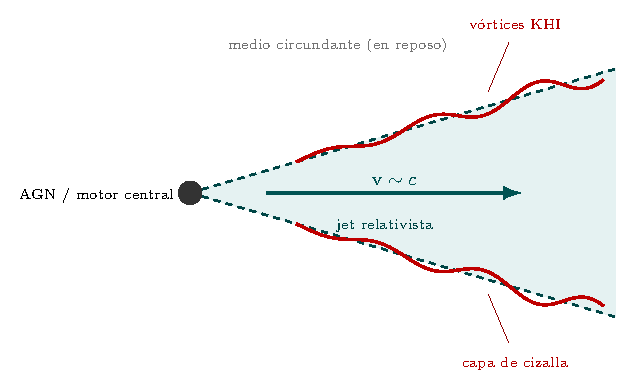
\includegraphics[width=0.96\linewidth,height=0.88\textheight,keepaspectratio]{contexto_jet.pdf}
\end{center}
\clearpage

\begin{center}
{\color{primary}\large\bfseries Figura 2}\quad{\small\color{accent}L\'amina 5}\quad{\small Dise\~no del Experimento Num\'erico: Dos Campa\~nas}\\[0.35cm]

\includegraphics[width=0.96\linewidth,height=0.88\textheight,keepaspectratio]{campana_A_3d.pdf}
\end{center}
\clearpage

\begin{center}
{\color{primary}\large\bfseries Figura 3}\quad{\small\color{accent}L\'amina 5}\quad{\small Dise\~no del Experimento Num\'erico: Dos Campa\~nas}\\[0.35cm]
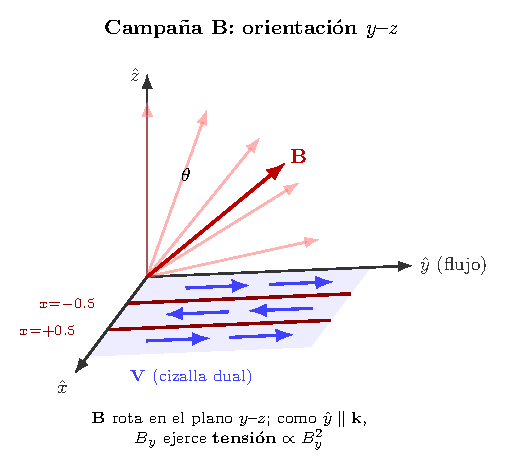
\includegraphics[width=0.96\linewidth,height=0.88\textheight,keepaspectratio]{campana_B_3d.pdf}
\end{center}
\clearpage

\begin{center}
{\color{primary}\large\bfseries Figura 4}\quad{\small\color{accent}L\'amina 5}\quad{\small Dise\~no del Experimento Num\'erico: Dos Campa\~nas}\\[0.35cm]

\includegraphics[width=0.96\linewidth,height=0.88\textheight,keepaspectratio]{campana_C_3d.pdf}
\end{center}
\clearpage

\begin{center}
{\color{primary}\large\bfseries Figura 5}\quad{\small\color{accent}L\'amina 8}\quad{\small Restricciones de Divergencia: el Sistema Aumentado GLM}\\[0.35cm]
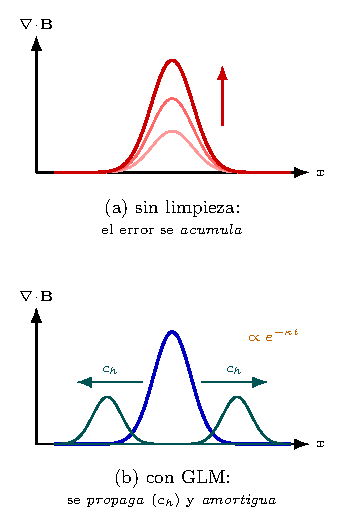
\includegraphics[width=0.96\linewidth,height=0.88\textheight,keepaspectratio]{glm_limpieza.pdf}
\end{center}
\clearpage

\begin{center}
{\color{primary}\large\bfseries Figura 6}\quad{\small\color{accent}L\'amina 12}\quad{\small Volumenes Finitos: la Formulaci\'on Integral Obligatoria}\\[0.35cm]
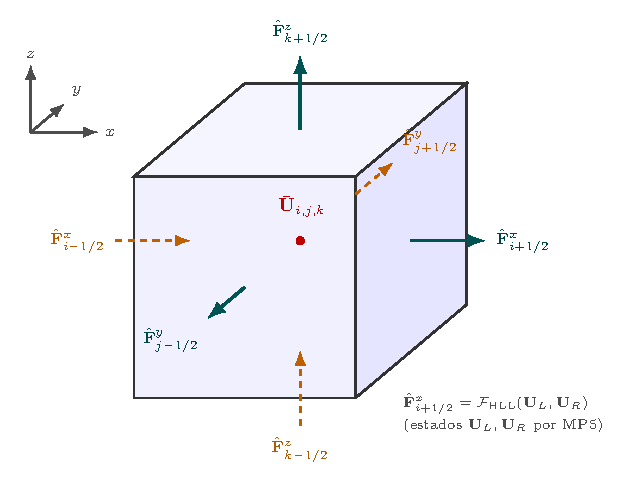
\includegraphics[width=0.96\linewidth,height=0.88\textheight,keepaspectratio]{celda_3d_flujos.pdf}
\end{center}
\clearpage

\begin{center}
{\color{primary}\large\bfseries Figura 7}\quad{\small\color{accent}L\'amina 13}\quad{\small Reconstrucci\'on MP5 $+$ Solucionador HLL}\\[0.35cm]
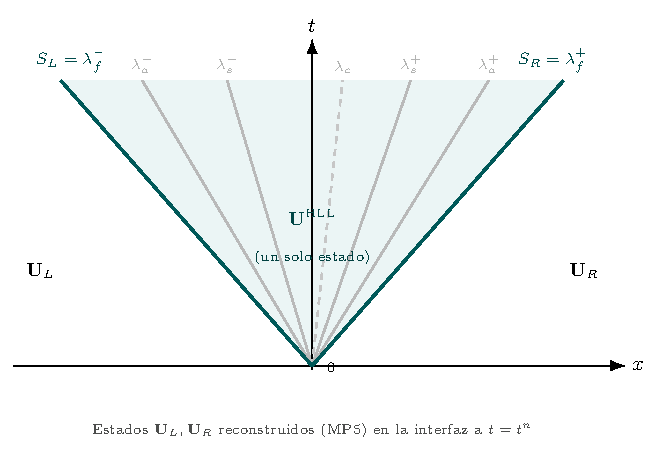
\includegraphics[width=0.96\linewidth,height=0.88\textheight,keepaspectratio]{riemann_hll.pdf}
\end{center}
\clearpage

\begin{center}
{\color{primary}\large\bfseries Figura 8}\quad{\small\color{accent}L\'amina 14}\quad{\small Rigidez Resistiva e Integraci\'on IMEX--RK}\\[0.35cm]
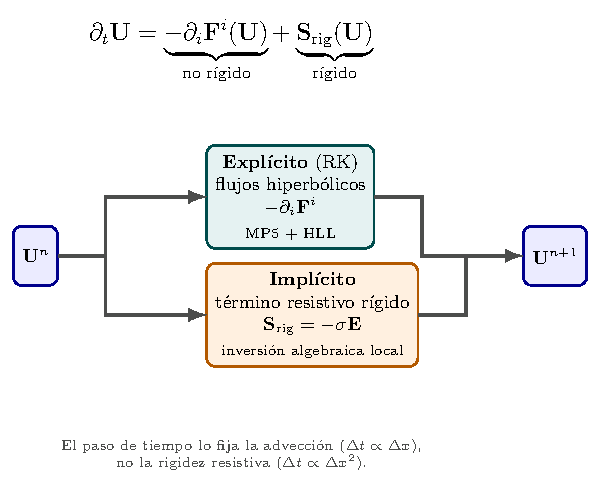
\includegraphics[width=0.96\linewidth,height=0.88\textheight,keepaspectratio]{imex_splitting_slide.pdf}
\end{center}
\clearpage

\begin{center}
{\color{primary}\large\bfseries Figura 9}\quad{\small\color{accent}L\'amina 16}\quad{\small Montaje Experimental: Doble Capa de Cizalla tipo Mizuno}\\[0.35cm]
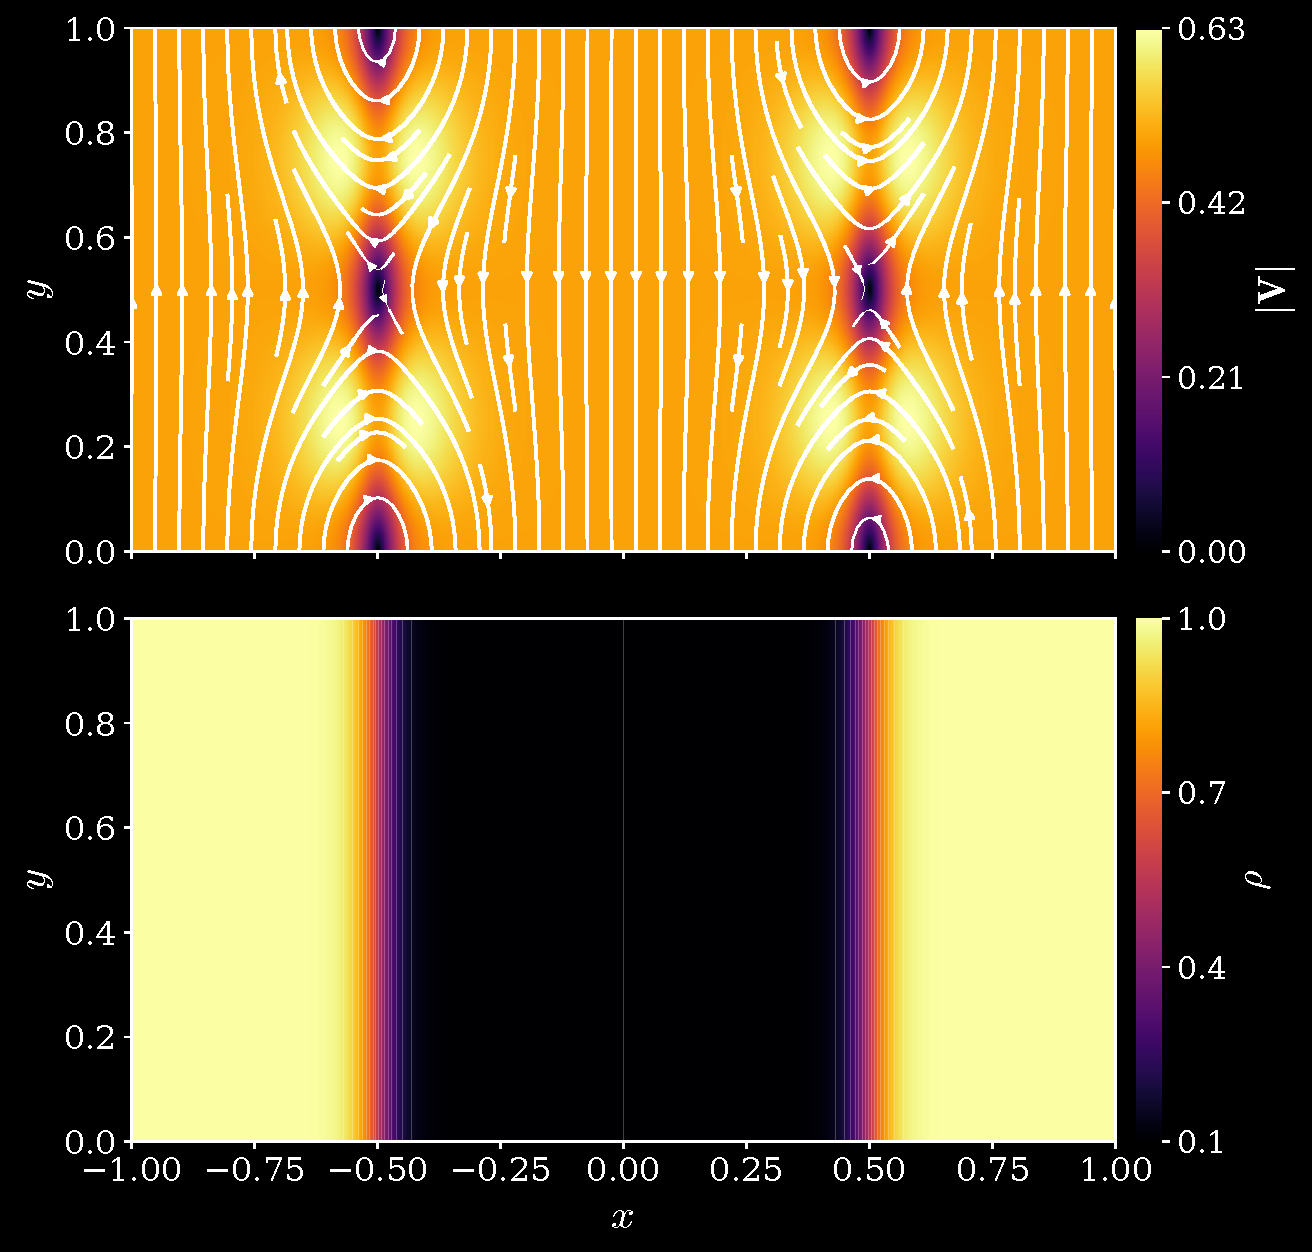
\includegraphics[width=0.96\linewidth,height=0.88\textheight,keepaspectratio]{setup_inicial_slide.pdf}
\end{center}
\clearpage

\begin{center}
{\color{primary}\large\bfseries Figura 10}\quad{\small\color{accent}L\'amina 18}\quad{\small El Barrido Completo en Conductividad}\\[0.35cm]
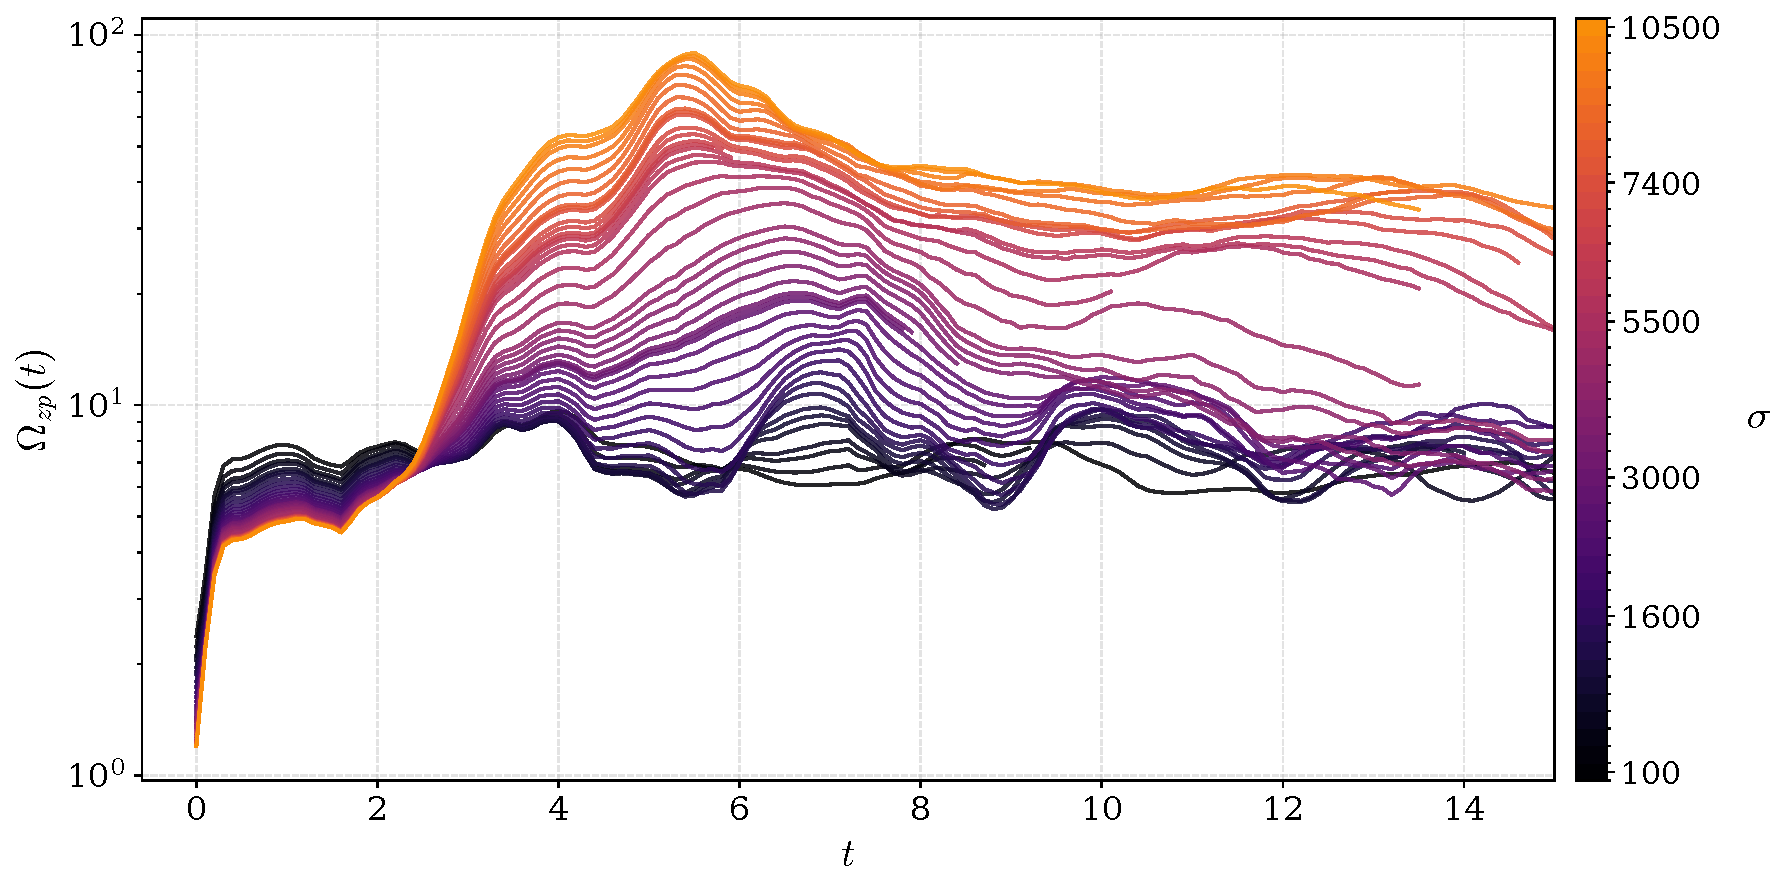
\includegraphics[width=0.96\linewidth,height=0.88\textheight,keepaspectratio]{fig_ultrawide_omega_zp_slide.pdf}
\end{center}
\clearpage

\begin{center}
{\color{primary}\large\bfseries Figura 11}\quad{\small\color{accent}L\'amina 19}\quad{\small Visi\'on Global del Barrido: Fenomenolog\'ia}\\[0.35cm]
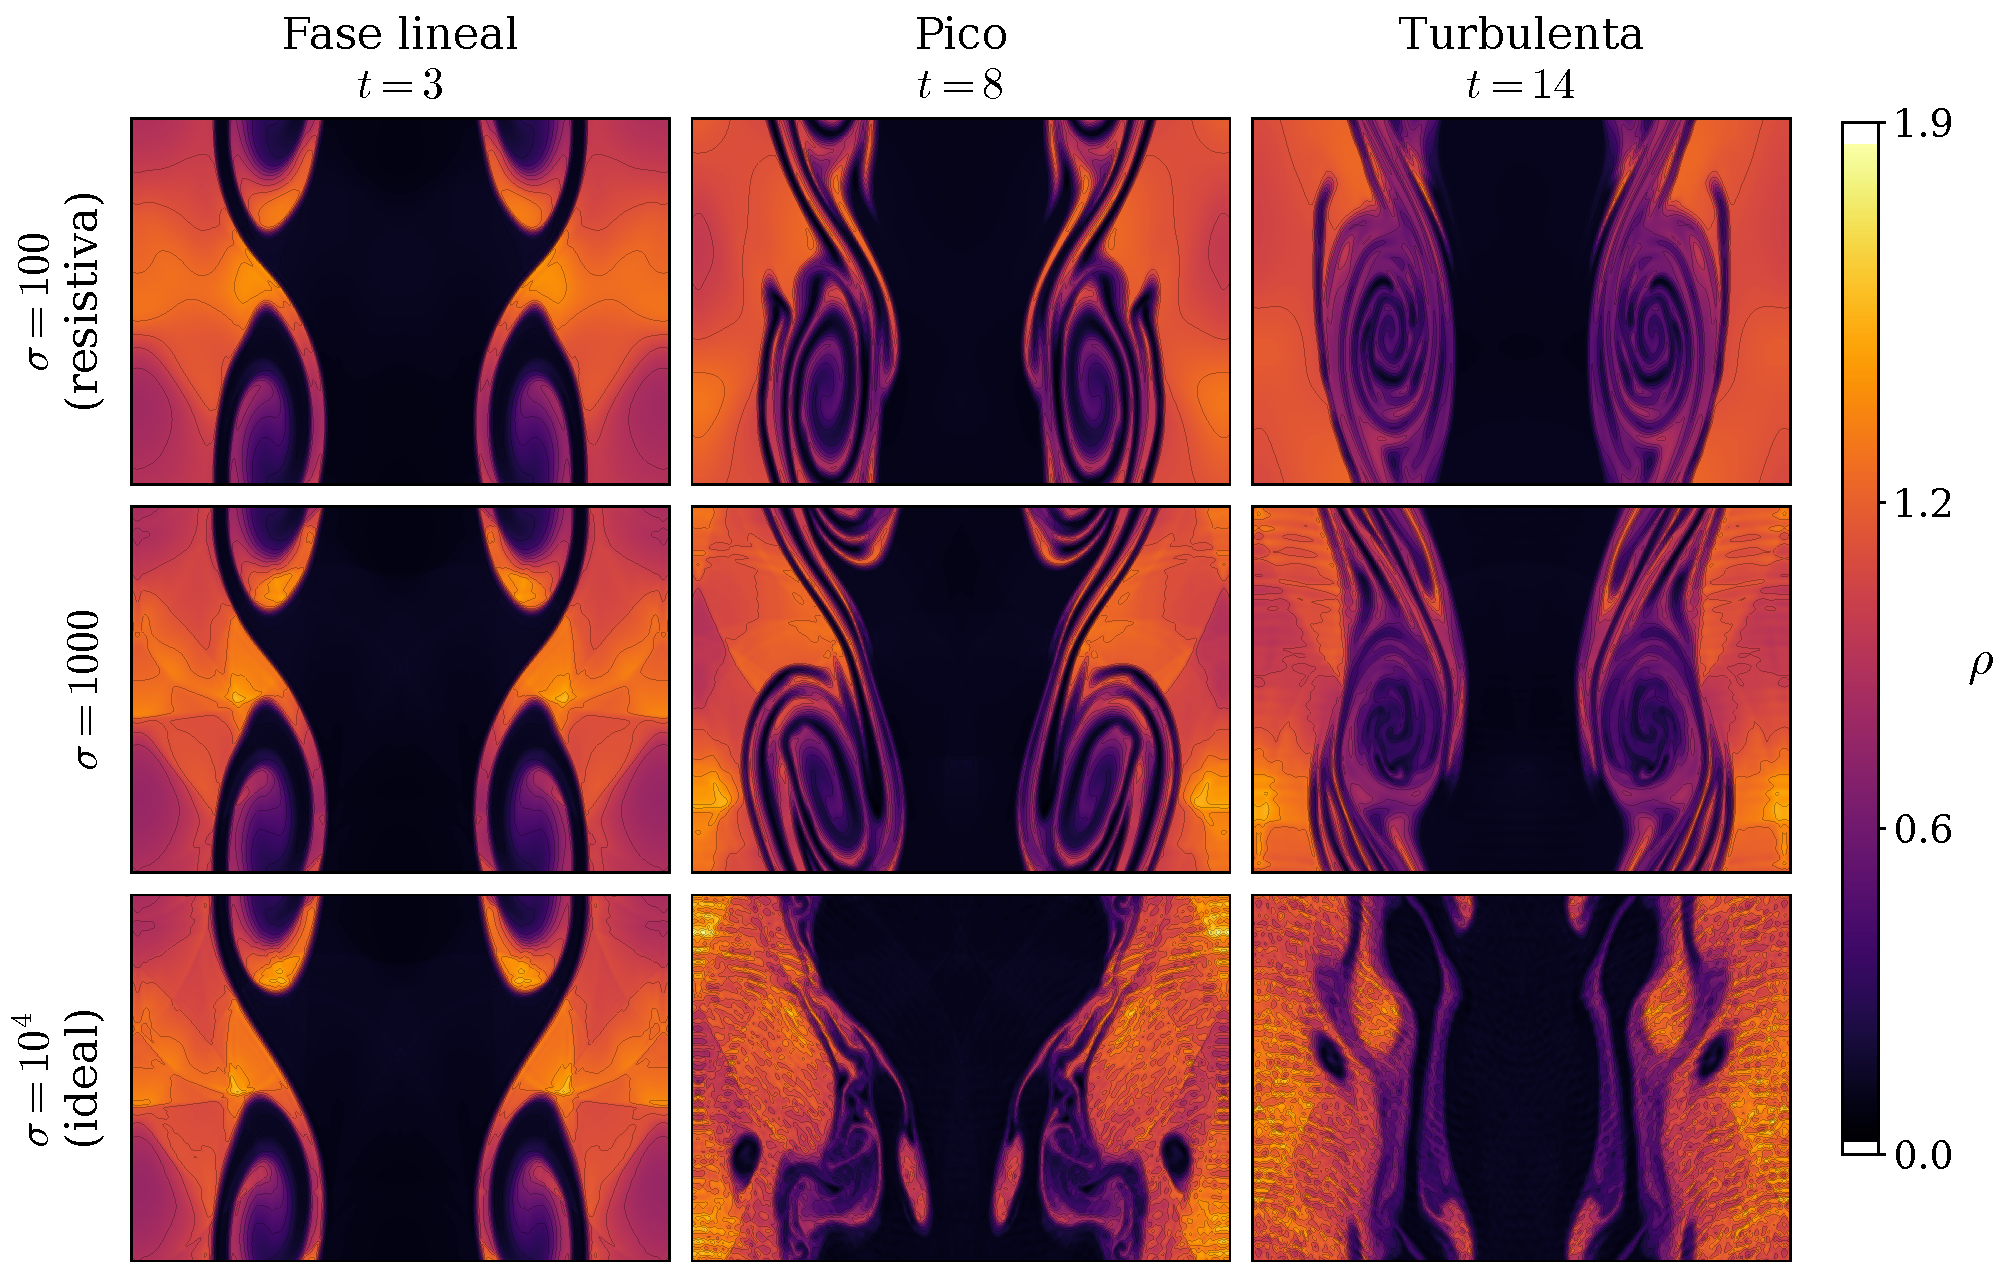
\includegraphics[width=0.96\linewidth,height=0.88\textheight,keepaspectratio]{fig_conductividad_rho_collage_slide.pdf}
\end{center}
\clearpage

\begin{center}
{\color{primary}\large\bfseries Figura 12}\quad{\small\color{accent}L\'amina 20}\quad{\small Extracci\'on de la Tasa de Crecimiento Lineal}\\[0.35cm]
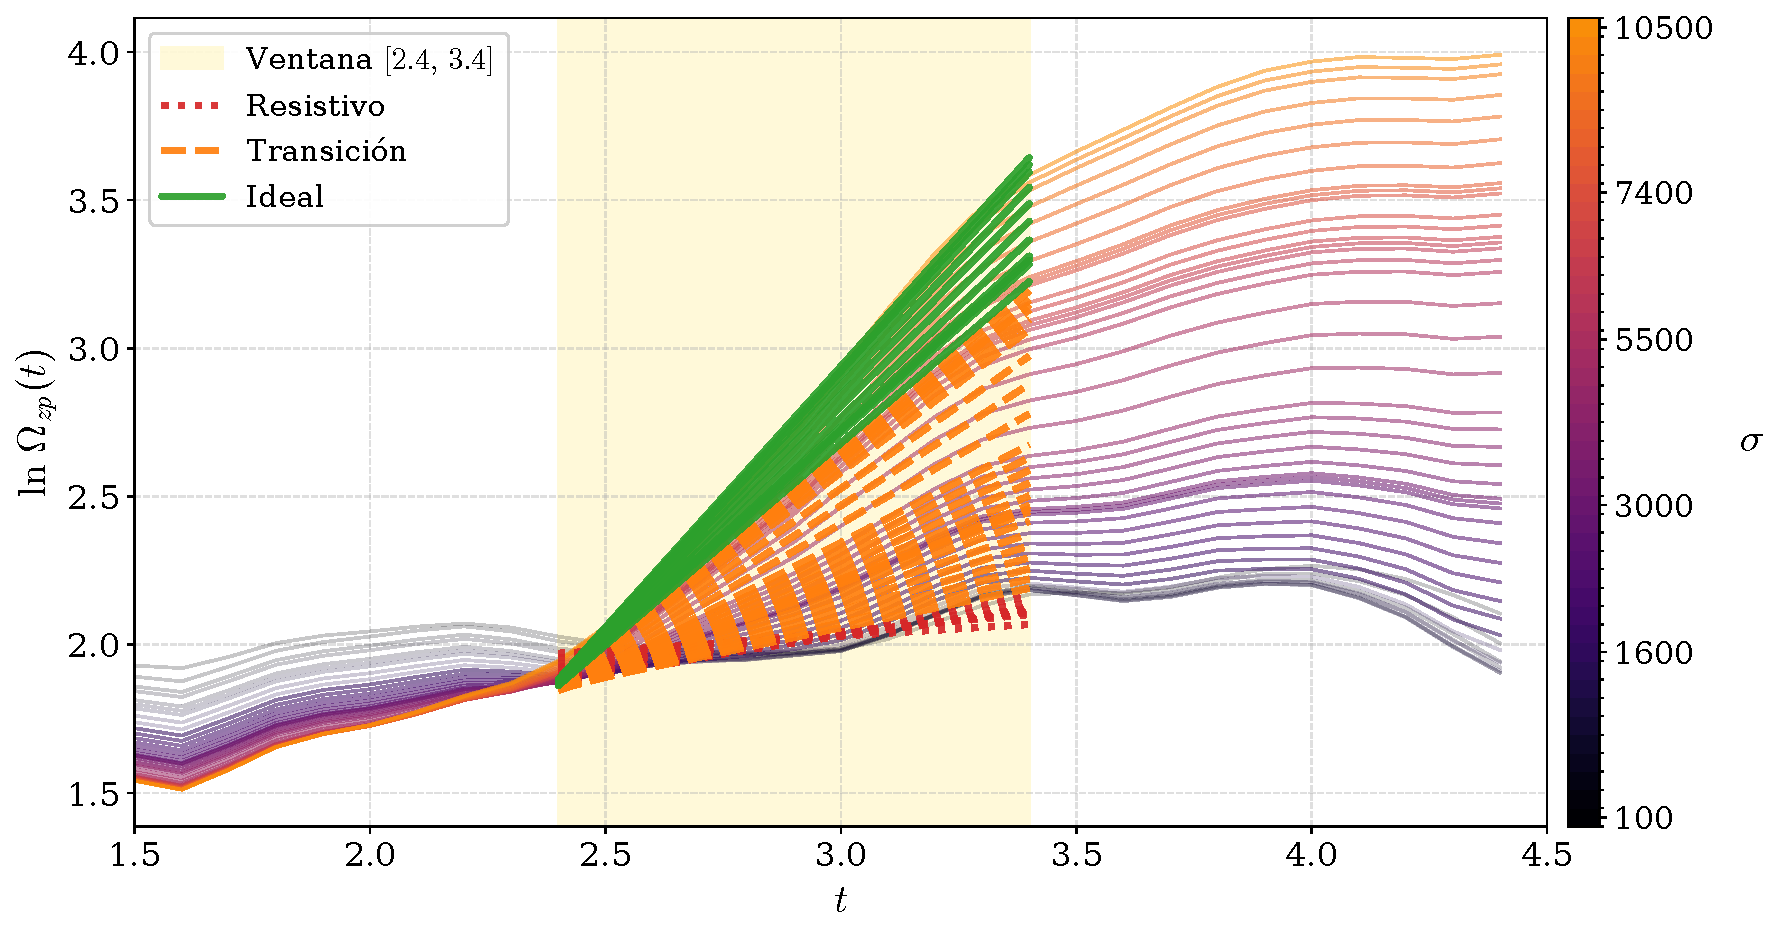
\includegraphics[width=0.96\linewidth,height=0.88\textheight,keepaspectratio]{ln_omega_vs_t_slide.pdf}
\end{center}
\clearpage

\begin{center}
{\color{primary}\large\bfseries Figura 13}\quad{\small\color{accent}L\'amina 21}\quad{\small La Transici\'on Resistivo$\,\to\,$Ideal: Sigmoide con \emph{Offset}}\\[0.35cm]

\includegraphics[width=0.96\linewidth,height=0.88\textheight,keepaspectratio]{fig1_ajuste_v6.pdf}
\end{center}
\clearpage

\begin{center}
{\color{primary}\large\bfseries Figura 14}\quad{\small\color{accent}L\'amina 22}\quad{\small Los Cuatro Estimadores de $\sigma_{\rm crit}$}\\[0.35cm]
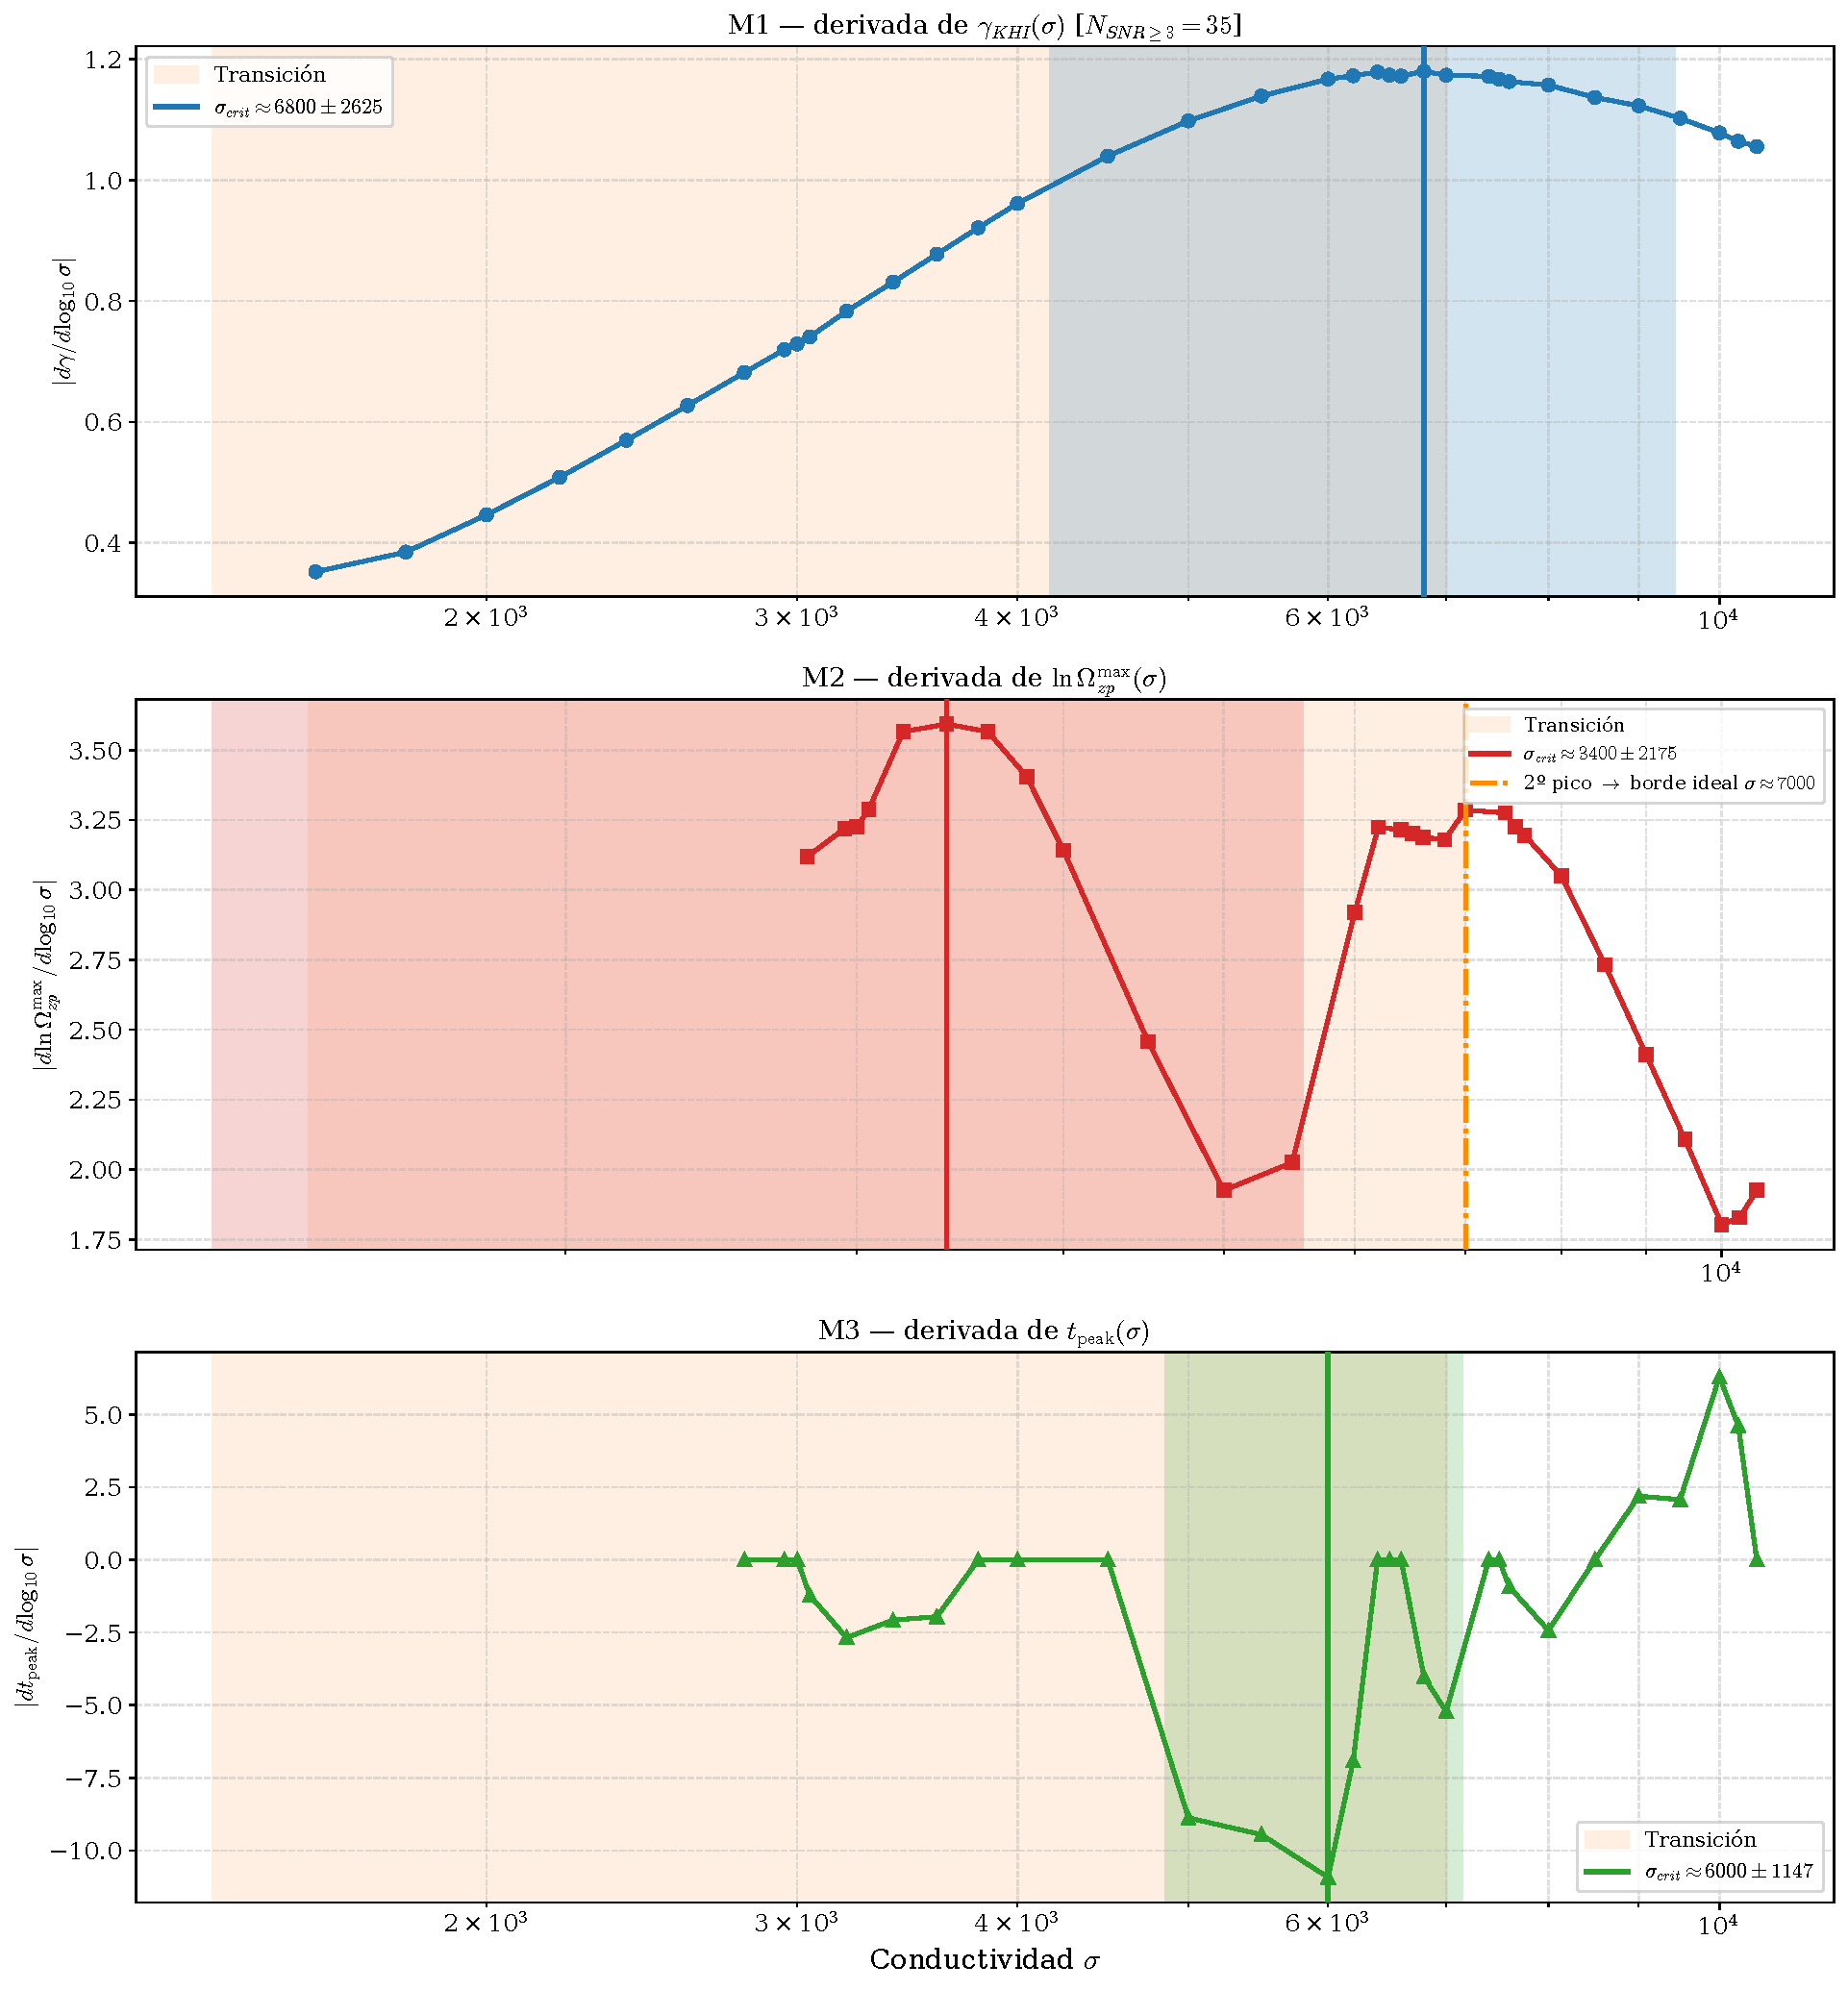
\includegraphics[width=0.96\linewidth,height=0.88\textheight,keepaspectratio]{fig_derivadas_scrit.pdf}
\end{center}
\clearpage

\begin{center}
{\color{primary}\large\bfseries Figura 15}\quad{\small\color{accent}L\'amina 22}\quad{\small Los Cuatro Estimadores de $\sigma_{\rm crit}$}\\[0.35cm]
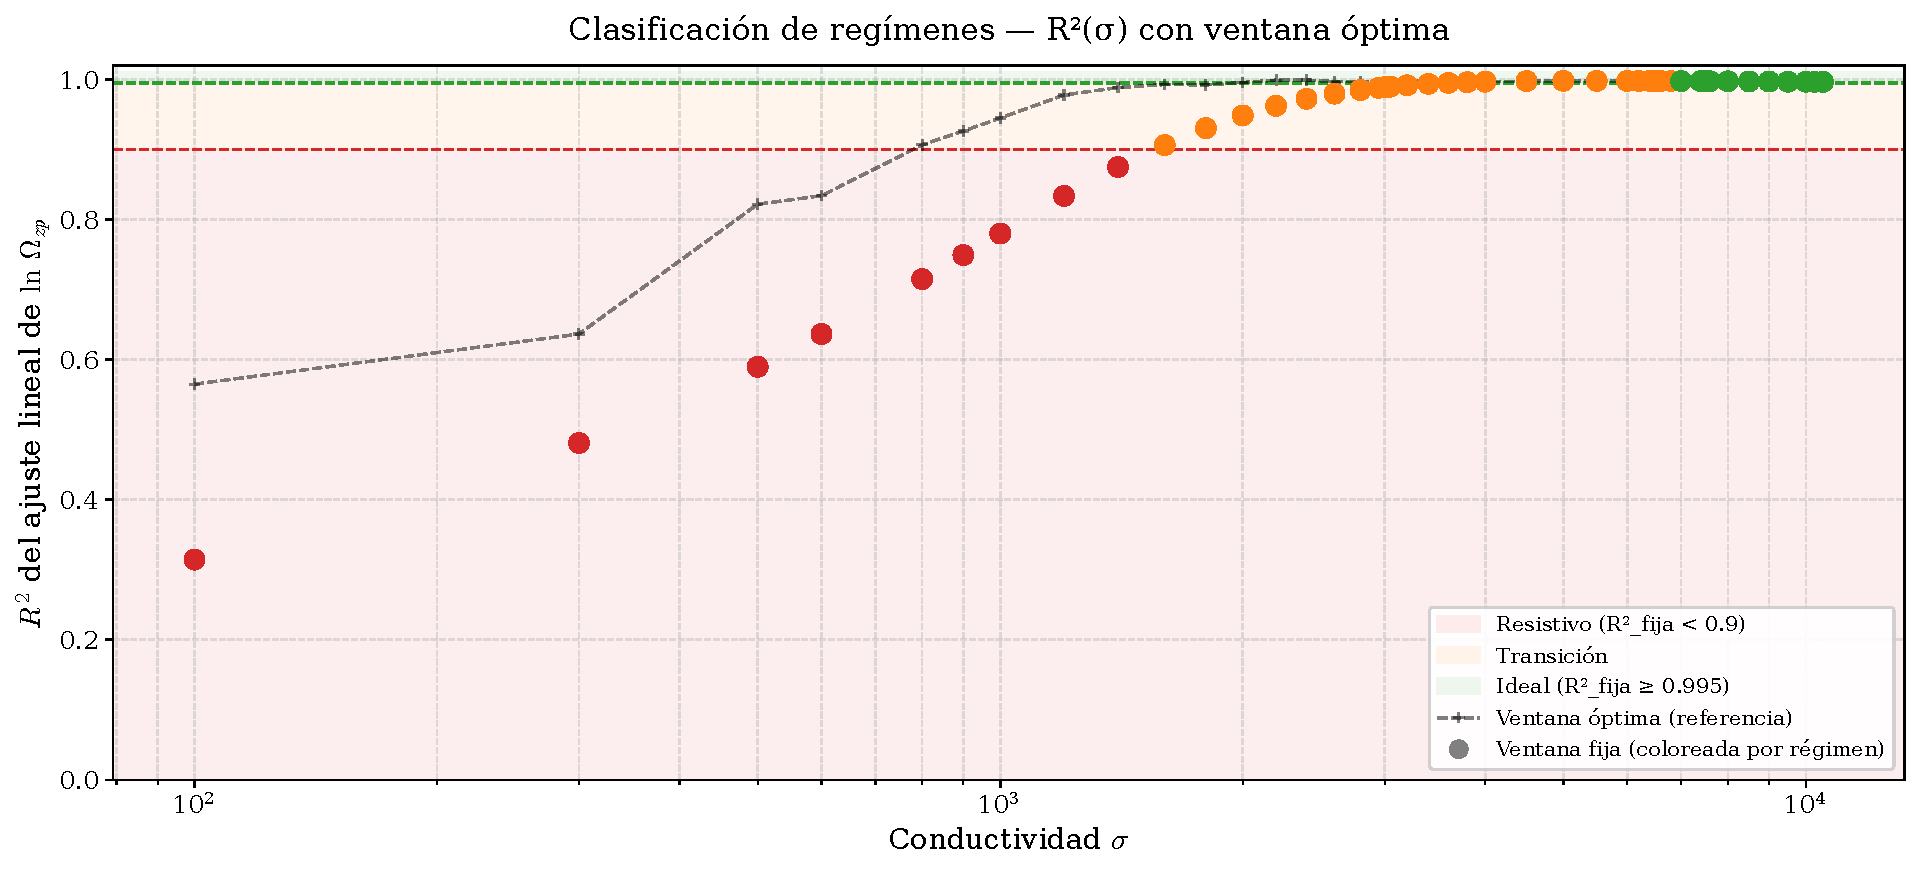
\includegraphics[width=0.96\linewidth,height=0.88\textheight,keepaspectratio]{fig_regimenes.pdf}
\end{center}
\clearpage

\begin{center}
{\color{primary}\large\bfseries Figura 16}\quad{\small\color{accent}L\'amina 23}\quad{\small $\sigma_{\rm crit}$ No Es un N\'umero: Es una Zona de Transici\'on}\\[0.35cm]
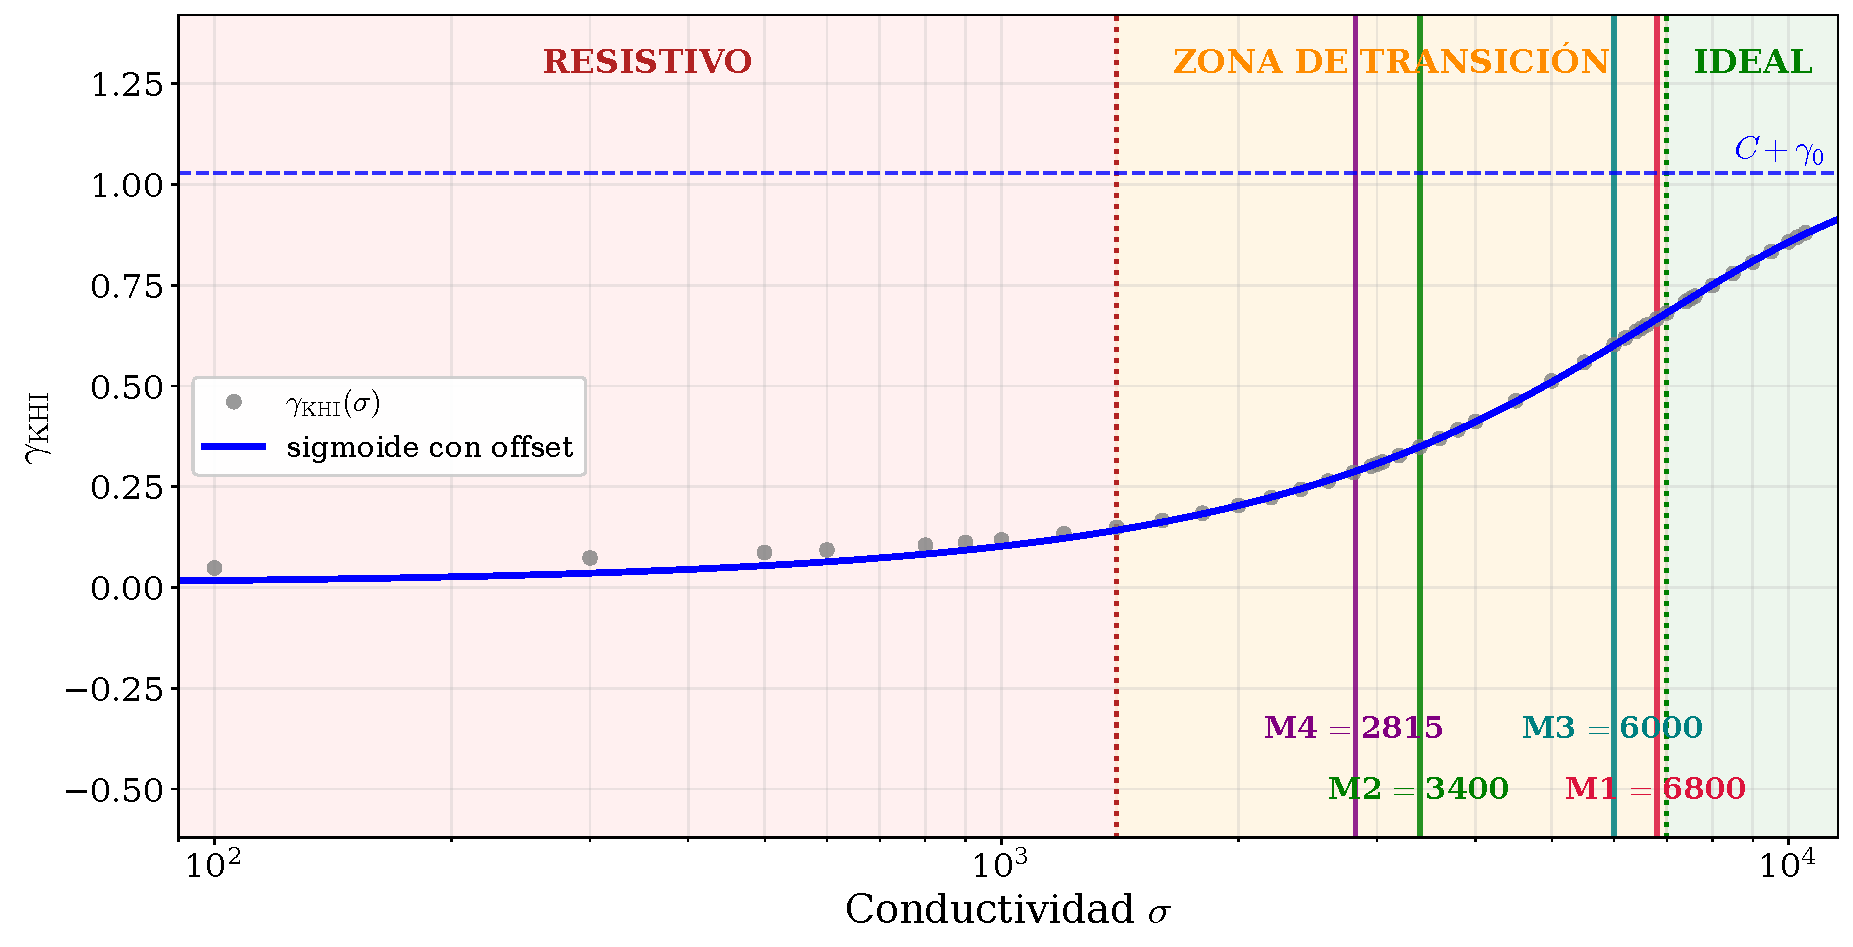
\includegraphics[width=0.96\linewidth,height=0.88\textheight,keepaspectratio]{fig_zona_transicion_slide.pdf}
\end{center}
\clearpage

\begin{center}
{\color{primary}\large\bfseries Figura 17}\quad{\small\color{accent}L\'amina 24}\quad{\small Contraste con la Teor\'ia Lineal: la Escalera de Predicciones}\\[0.35cm]
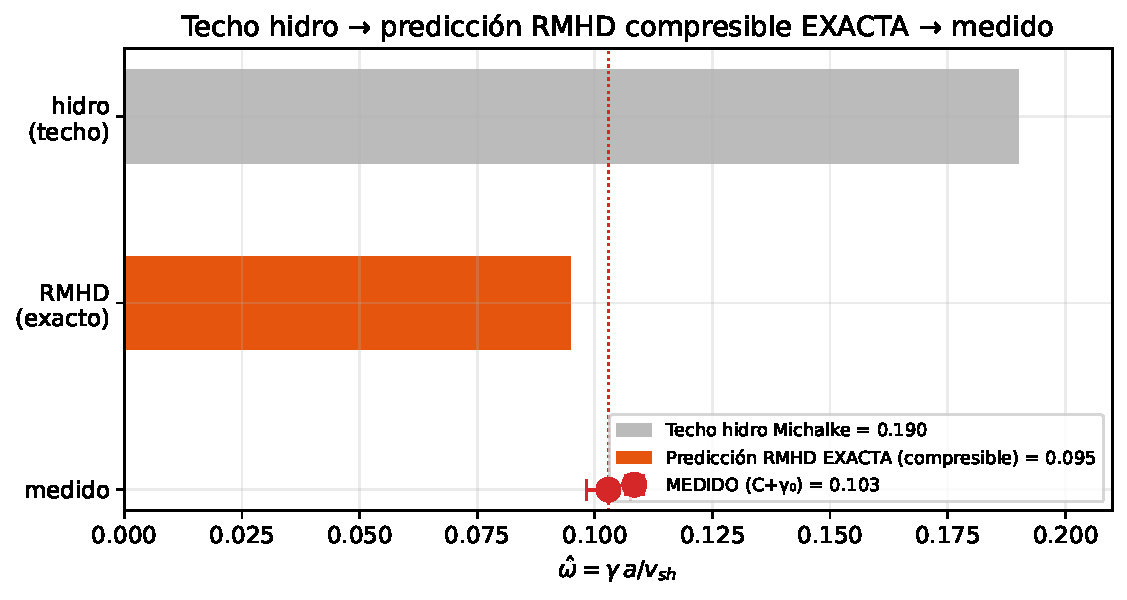
\includegraphics[width=0.96\linewidth,height=0.88\textheight,keepaspectratio]{fig6_escalera.pdf}
\end{center}
\clearpage

\begin{center}
{\color{primary}\large\bfseries Figura 18}\quad{\small\color{accent}L\'amina 25}\quad{\small No Linealidad: Ley de Potencia de la Enstrof\'ia M\'axima}\\[0.35cm]
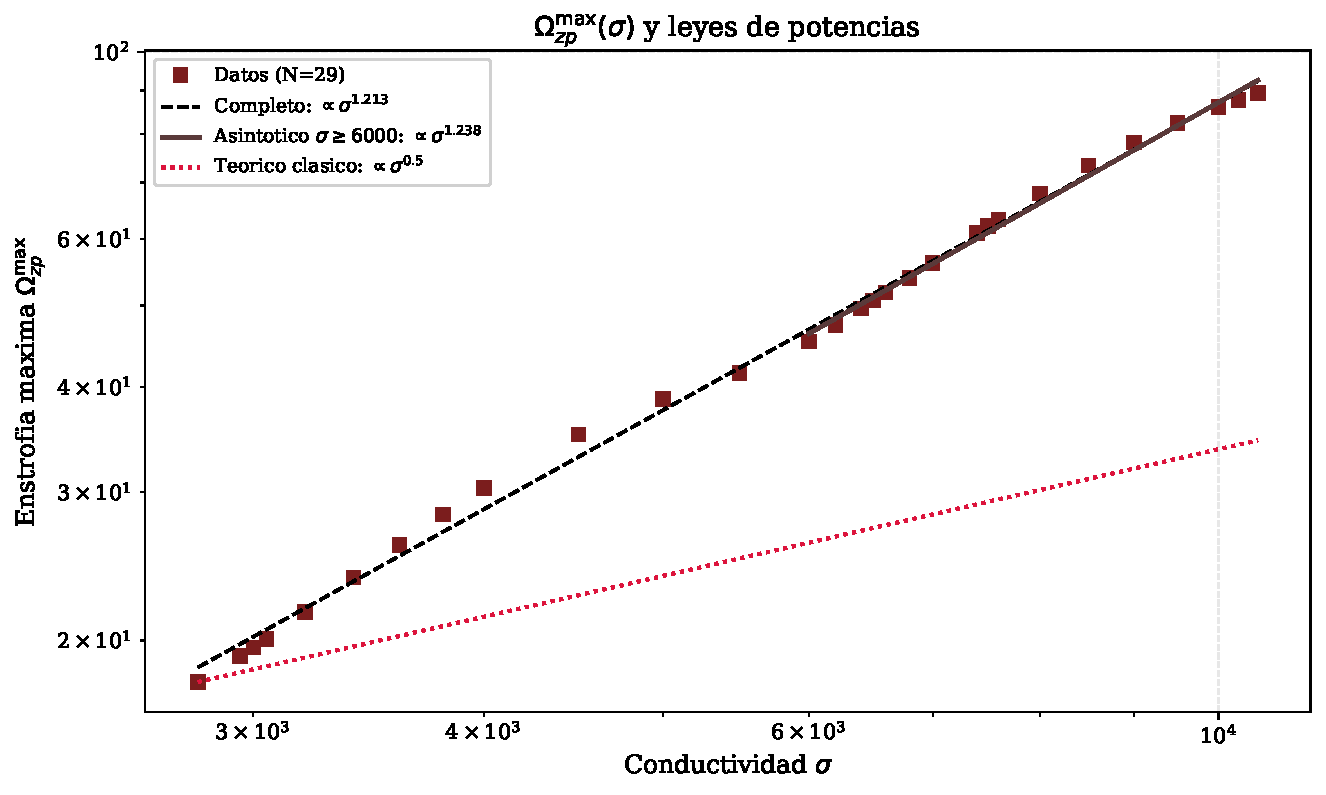
\includegraphics[width=0.96\linewidth,height=0.88\textheight,keepaspectratio]{fig_omega_max_leypotencias.pdf}
\end{center}
\clearpage

\begin{center}
{\color{primary}\large\bfseries Figura 19}\quad{\small\color{accent}L\'amina 26}\quad{\small Variables Globales: la Firma Electromagn\'etica de $\sigma$}\\[0.35cm]
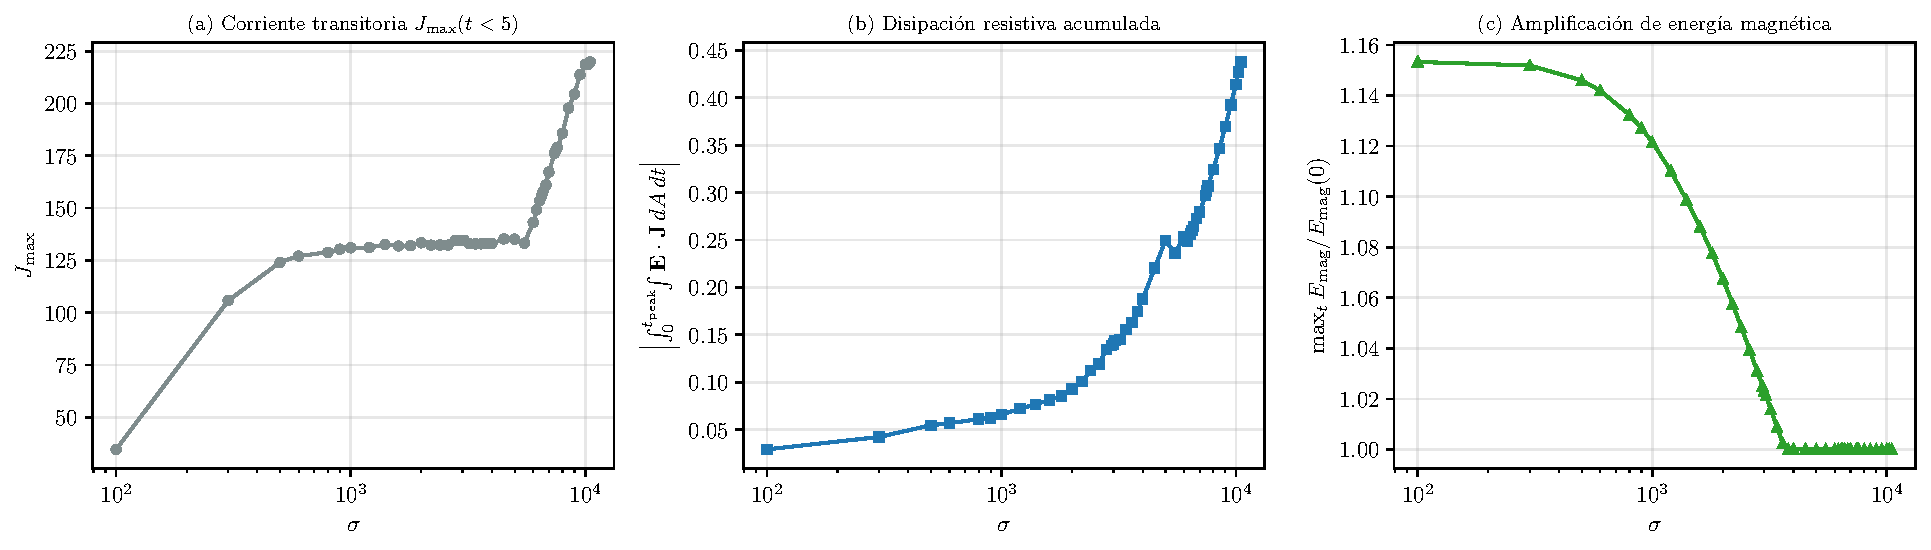
\includegraphics[width=0.96\linewidth,height=0.88\textheight,keepaspectratio]{fig_global_campos_transitorio.pdf}
\end{center}
\clearpage

\begin{center}
{\color{primary}\large\bfseries Figura 20}\quad{\small\color{accent}L\'amina 27}\quad{\small Campa\~na Magn\'etica I: Intensidad y Orientaci\'on}\\[0.35cm]
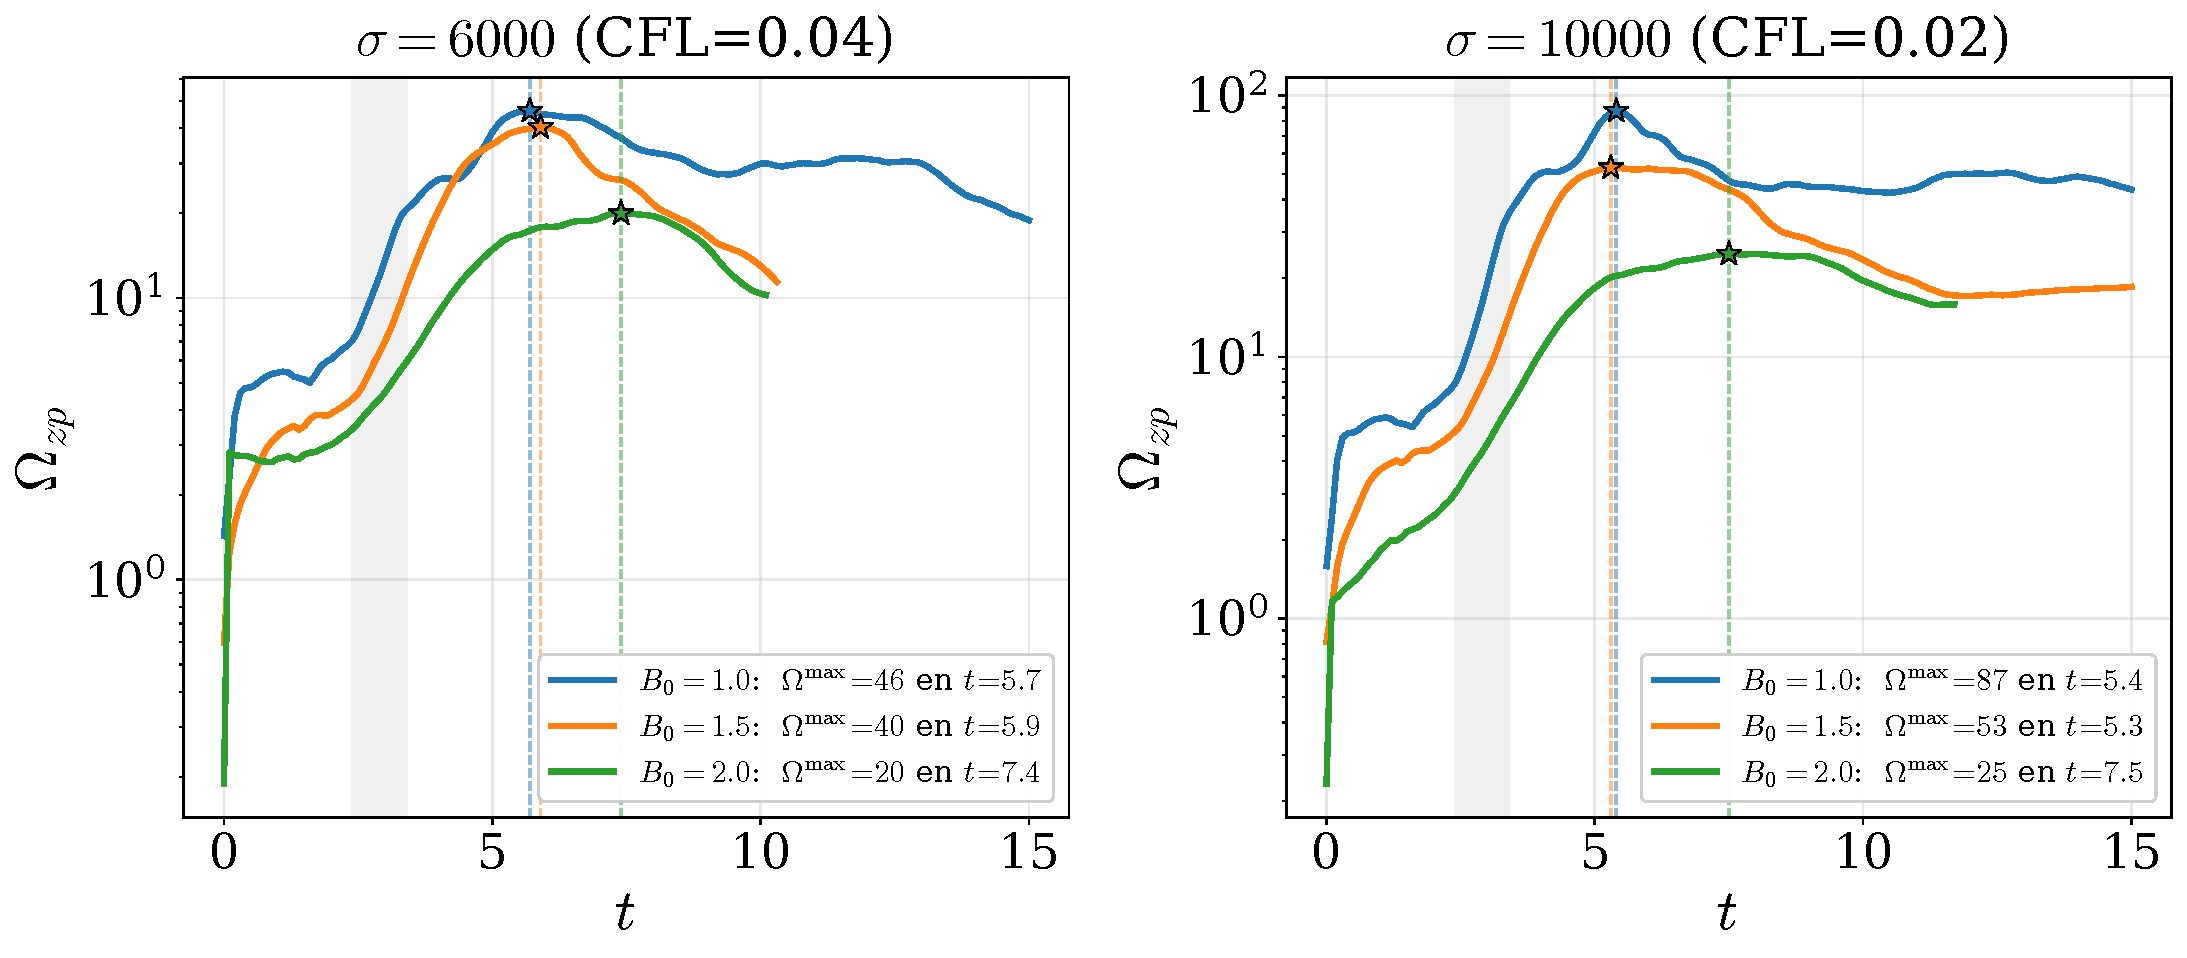
\includegraphics[width=0.96\linewidth,height=0.88\textheight,keepaspectratio]{fig_campA_enstrofia_slide.pdf}
\end{center}
\clearpage

\begin{center}
{\color{primary}\large\bfseries Figura 21}\quad{\small\color{accent}L\'amina 27}\quad{\small Campa\~na Magn\'etica I: Intensidad y Orientaci\'on}\\[0.35cm]
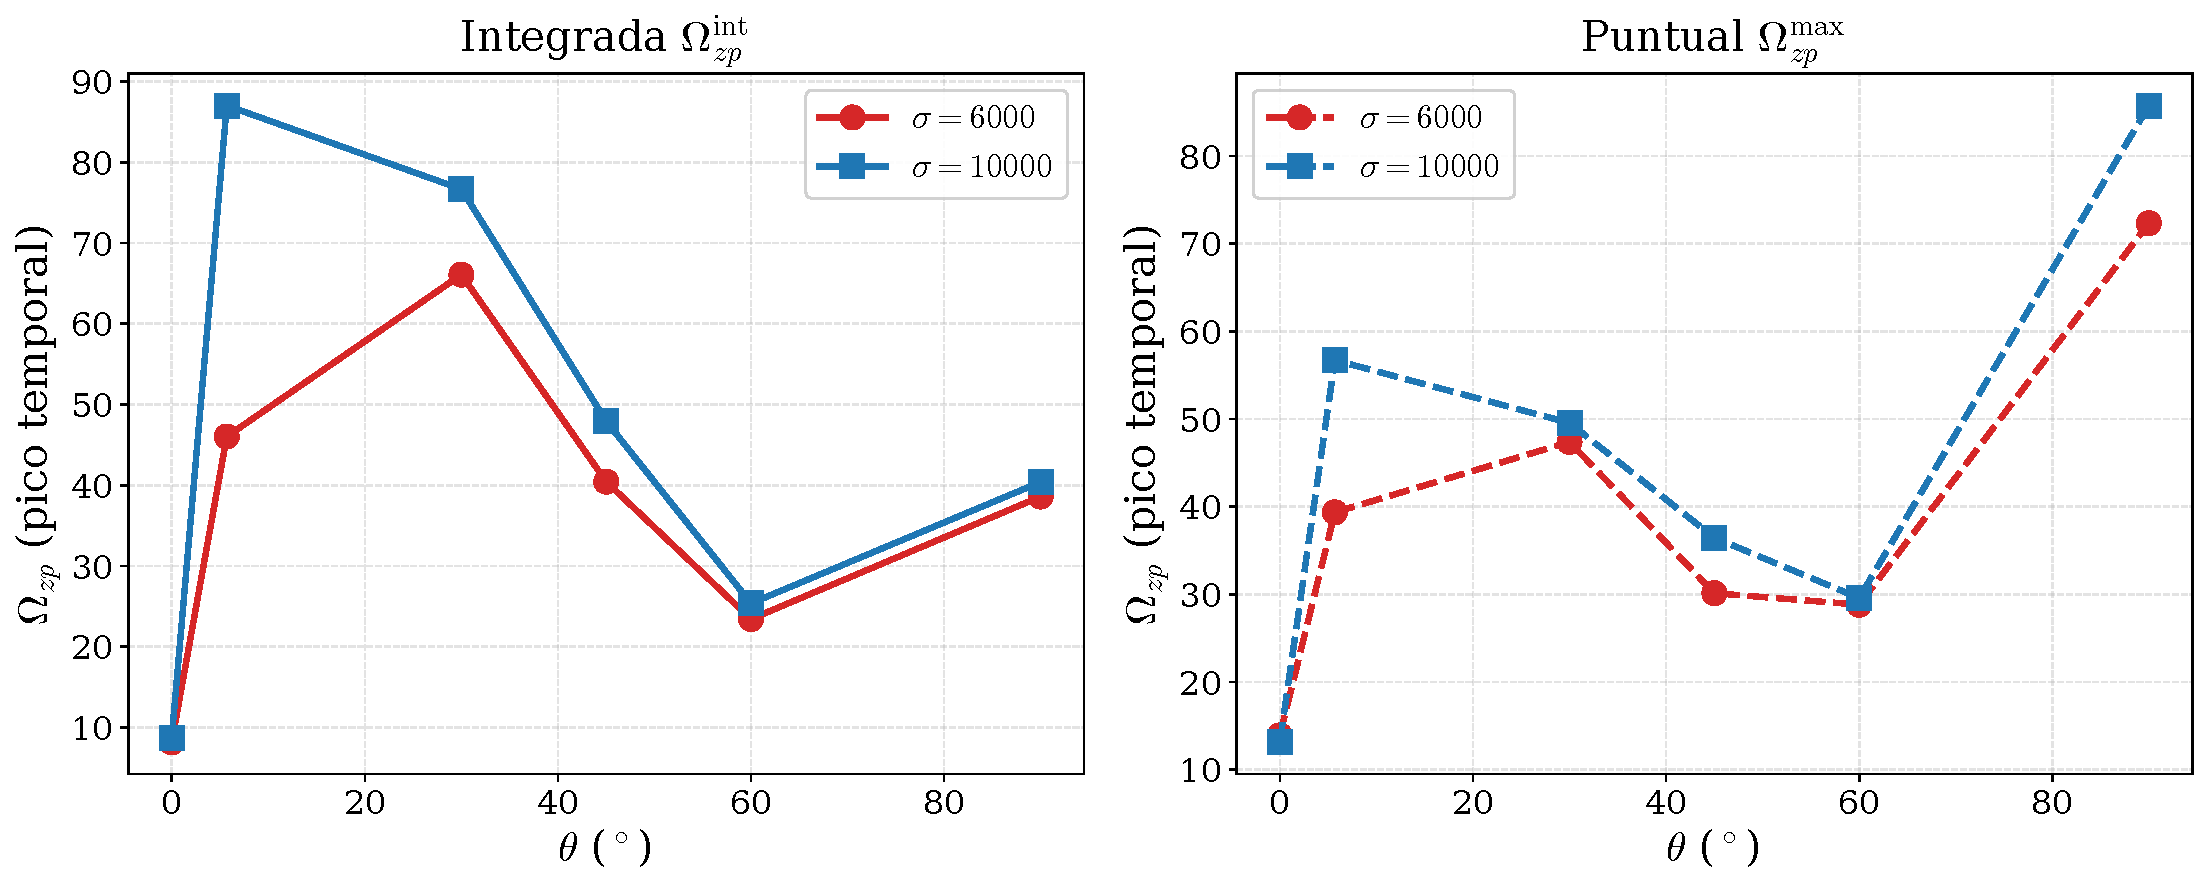
\includegraphics[width=0.96\linewidth,height=0.88\textheight,keepaspectratio]{fig_campB_omegamax_theta_slide.pdf}
\end{center}
\clearpage

\begin{center}
{\color{primary}\large\bfseries Figura 22}\quad{\small\color{accent}L\'amina 28}\quad{\small Campa\~na Magn\'etica II: Balance Energ\'etico y Canales de Disipaci\'on}\\[0.35cm]
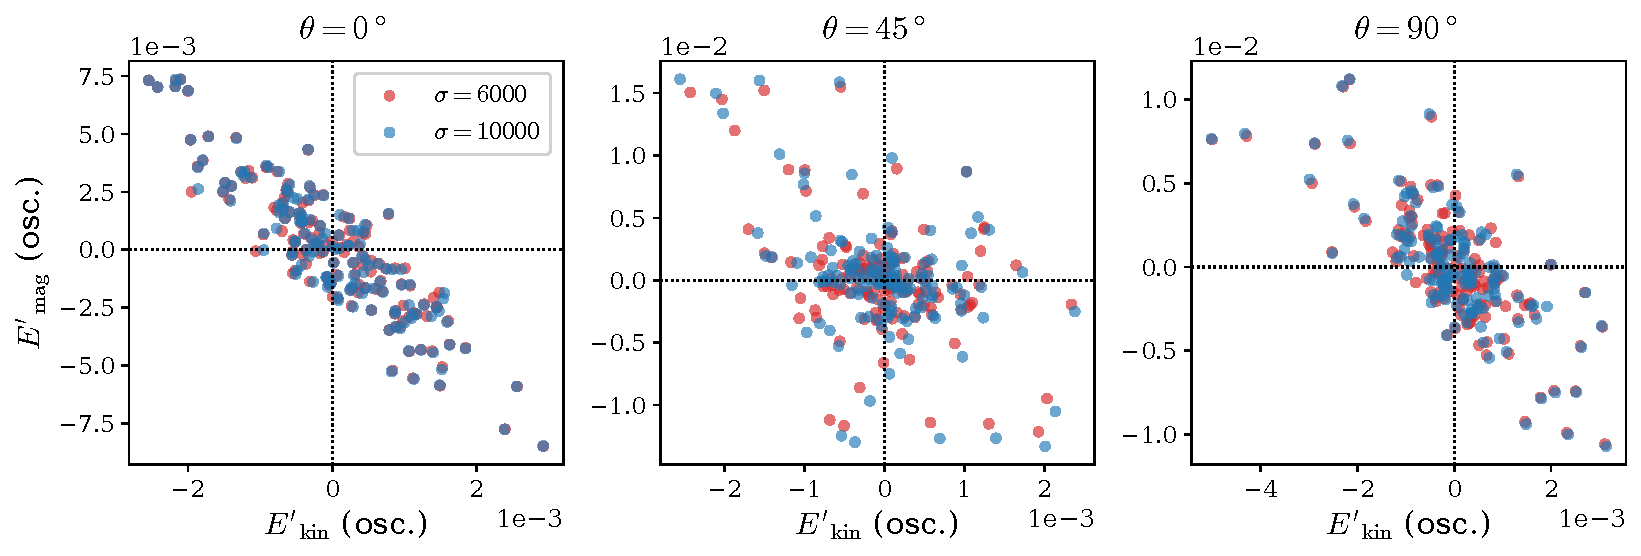
\includegraphics[width=0.96\linewidth,height=0.88\textheight,keepaspectratio]{fig_campB_ekin_emag_scatter_slide.pdf}
\end{center}
\clearpage

\begin{center}
{\color{primary}\large\bfseries Figura 23}\quad{\small\color{accent}L\'amina 29}\quad{\small Campa\~na Magn\'etica III: Orientaci\'on sin Tensi\'on (plano $x$--$z$)}\\[0.35cm]
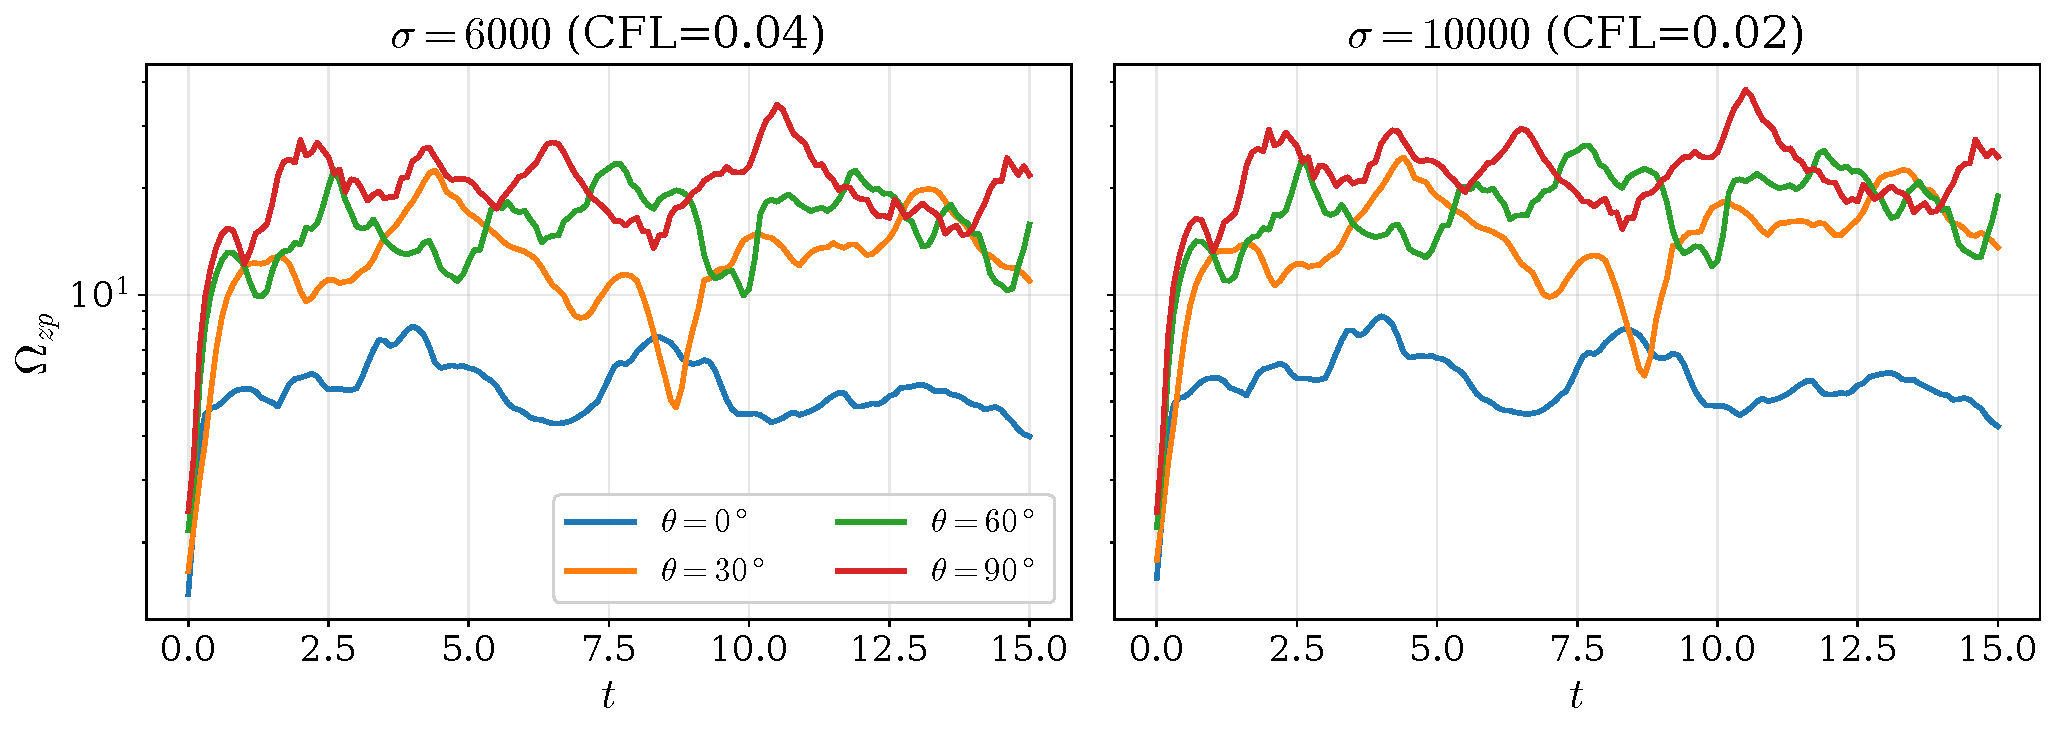
\includegraphics[width=0.96\linewidth,height=0.88\textheight,keepaspectratio]{fig_campC_enstrofia_slide.pdf}
\end{center}
\clearpage

\begin{center}
{\color{primary}\large\bfseries Figura 24}\quad{\small\color{accent}L\'amina 29}\quad{\small Campa\~na Magn\'etica III: Orientaci\'on sin Tensi\'on (plano $x$--$z$)}\\[0.35cm]
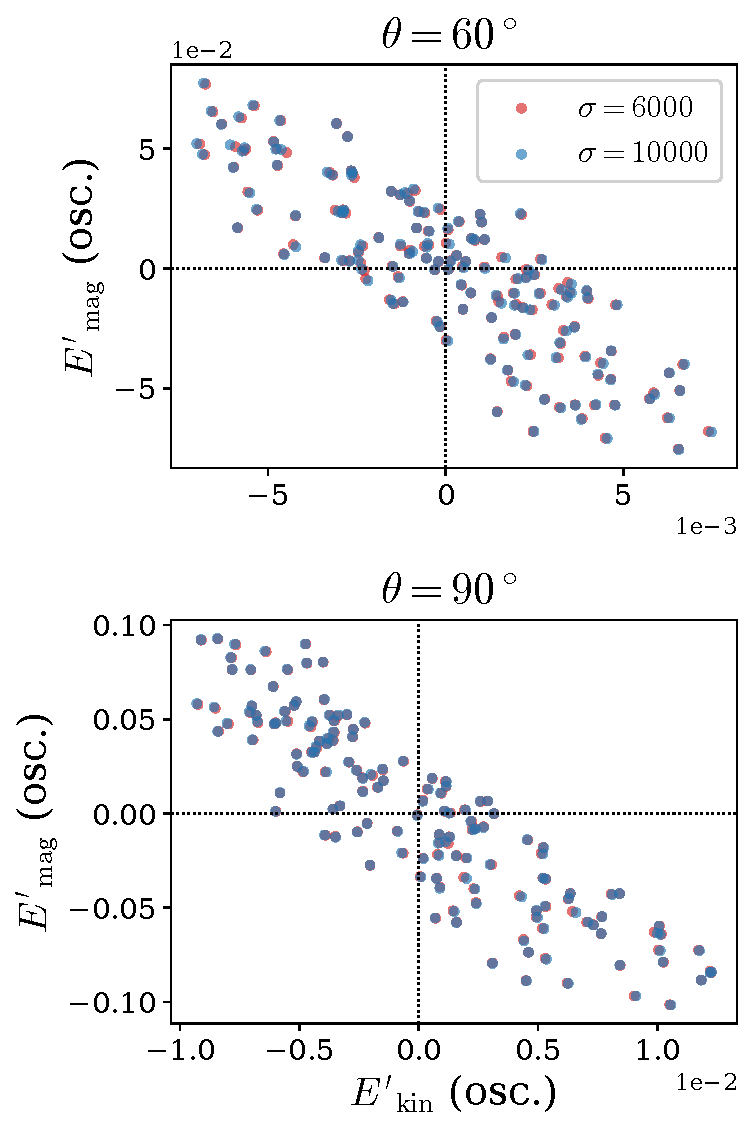
\includegraphics[width=0.96\linewidth,height=0.88\textheight,keepaspectratio]{fig_campC_ekin_emag_scatter_slide.pdf}
\end{center}
\clearpage

\begin{center}
{\color{primary}\large\bfseries Figura 25}\quad{\small\color{accent}Respaldo B5}\quad{\small B5 · Proyecci\'on 3+1 de la Ley de Ohm --- \'Algebra Completa}\\[0.35cm]

\includegraphics[width=0.96\linewidth,height=0.88\textheight,keepaspectratio]{marco_comovil_lab.pdf}
\end{center}
\clearpage

\begin{center}
{\color{primary}\large\bfseries Figura 26}\quad{\small\color{accent}Respaldo B6}\quad{\small B6 · Validaci\'on del Solucionador de la Teor\'ia Lineal}\\[0.35cm]
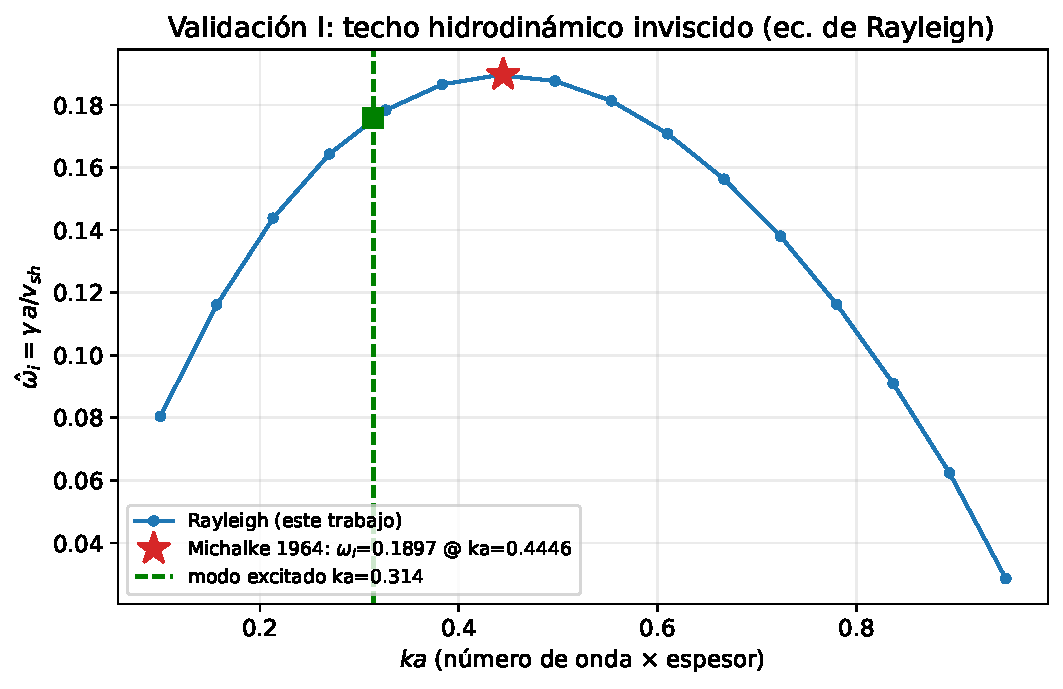
\includegraphics[width=0.96\linewidth,height=0.88\textheight,keepaspectratio]{fig4_michalke.pdf}
\end{center}
\clearpage

\begin{center}
{\color{primary}\large\bfseries Figura 27}\quad{\small\color{accent}Respaldo B6}\quad{\small B6 · Validaci\'on del Solucionador de la Teor\'ia Lineal}\\[0.35cm]
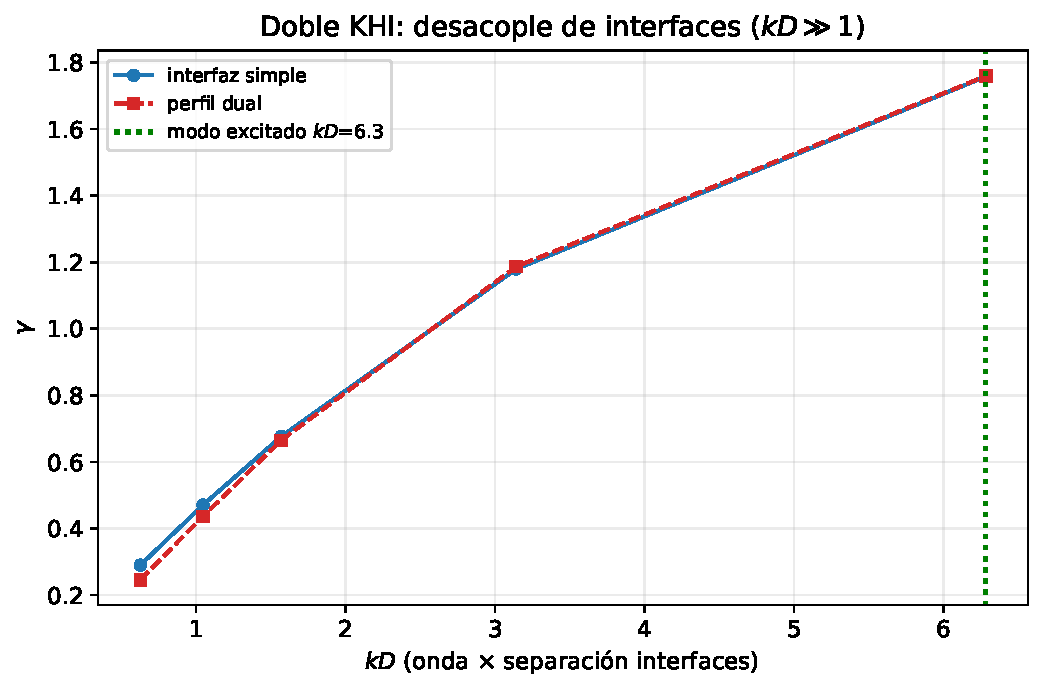
\includegraphics[width=0.96\linewidth,height=0.88\textheight,keepaspectratio]{fig7_dual.pdf}
\end{center}
\clearpage

\begin{center}
{\color{primary}\large\bfseries Figura 28}\quad{\small\color{accent}Respaldo B8}\quad{\small B8 · Estad\'istica del Ajuste Sigmoide}\\[0.35cm]
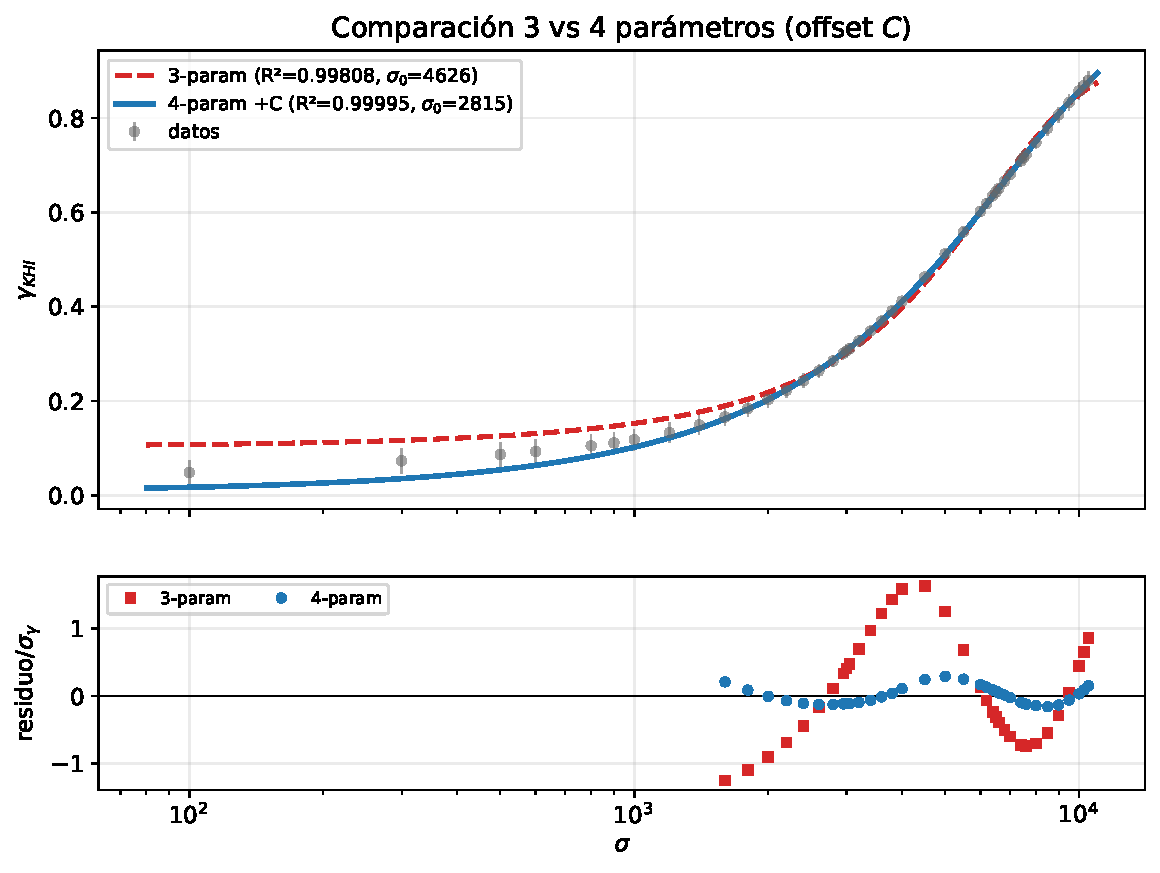
\includegraphics[width=0.96\linewidth,height=0.88\textheight,keepaspectratio]{fig2_3p_vs_4p.pdf}
\end{center}
\clearpage

\begin{center}
{\color{primary}\large\bfseries Figura 29}\quad{\small\color{accent}Respaldo B8}\quad{\small B8 · Estad\'istica del Ajuste Sigmoide}\\[0.35cm]

\includegraphics[width=0.96\linewidth,height=0.88\textheight,keepaspectratio]{fig10_holdout.pdf}
\end{center}
\clearpage

\begin{center}
{\color{primary}\large\bfseries Figura 30}\quad{\small\color{accent}Respaldo B11}\quad{\small B11 · Estructuras Secundarias y Campa\~na C}\\[0.35cm]
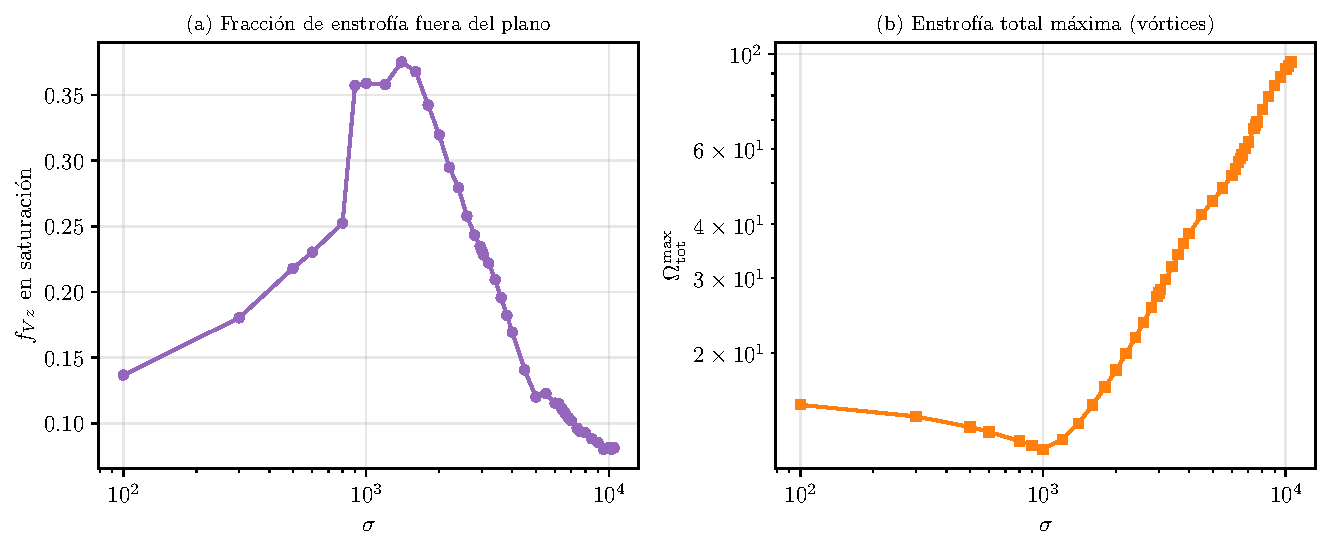
\includegraphics[width=0.96\linewidth,height=0.88\textheight,keepaspectratio]{fig_global_estructuras.pdf}
\end{center}
\clearpage

\begin{center}
{\color{primary}\large\bfseries Figura 31}\quad{\small\color{accent}Respaldo B11}\quad{\small B11 · Estructuras Secundarias y Campa\~na C}\\[0.35cm]
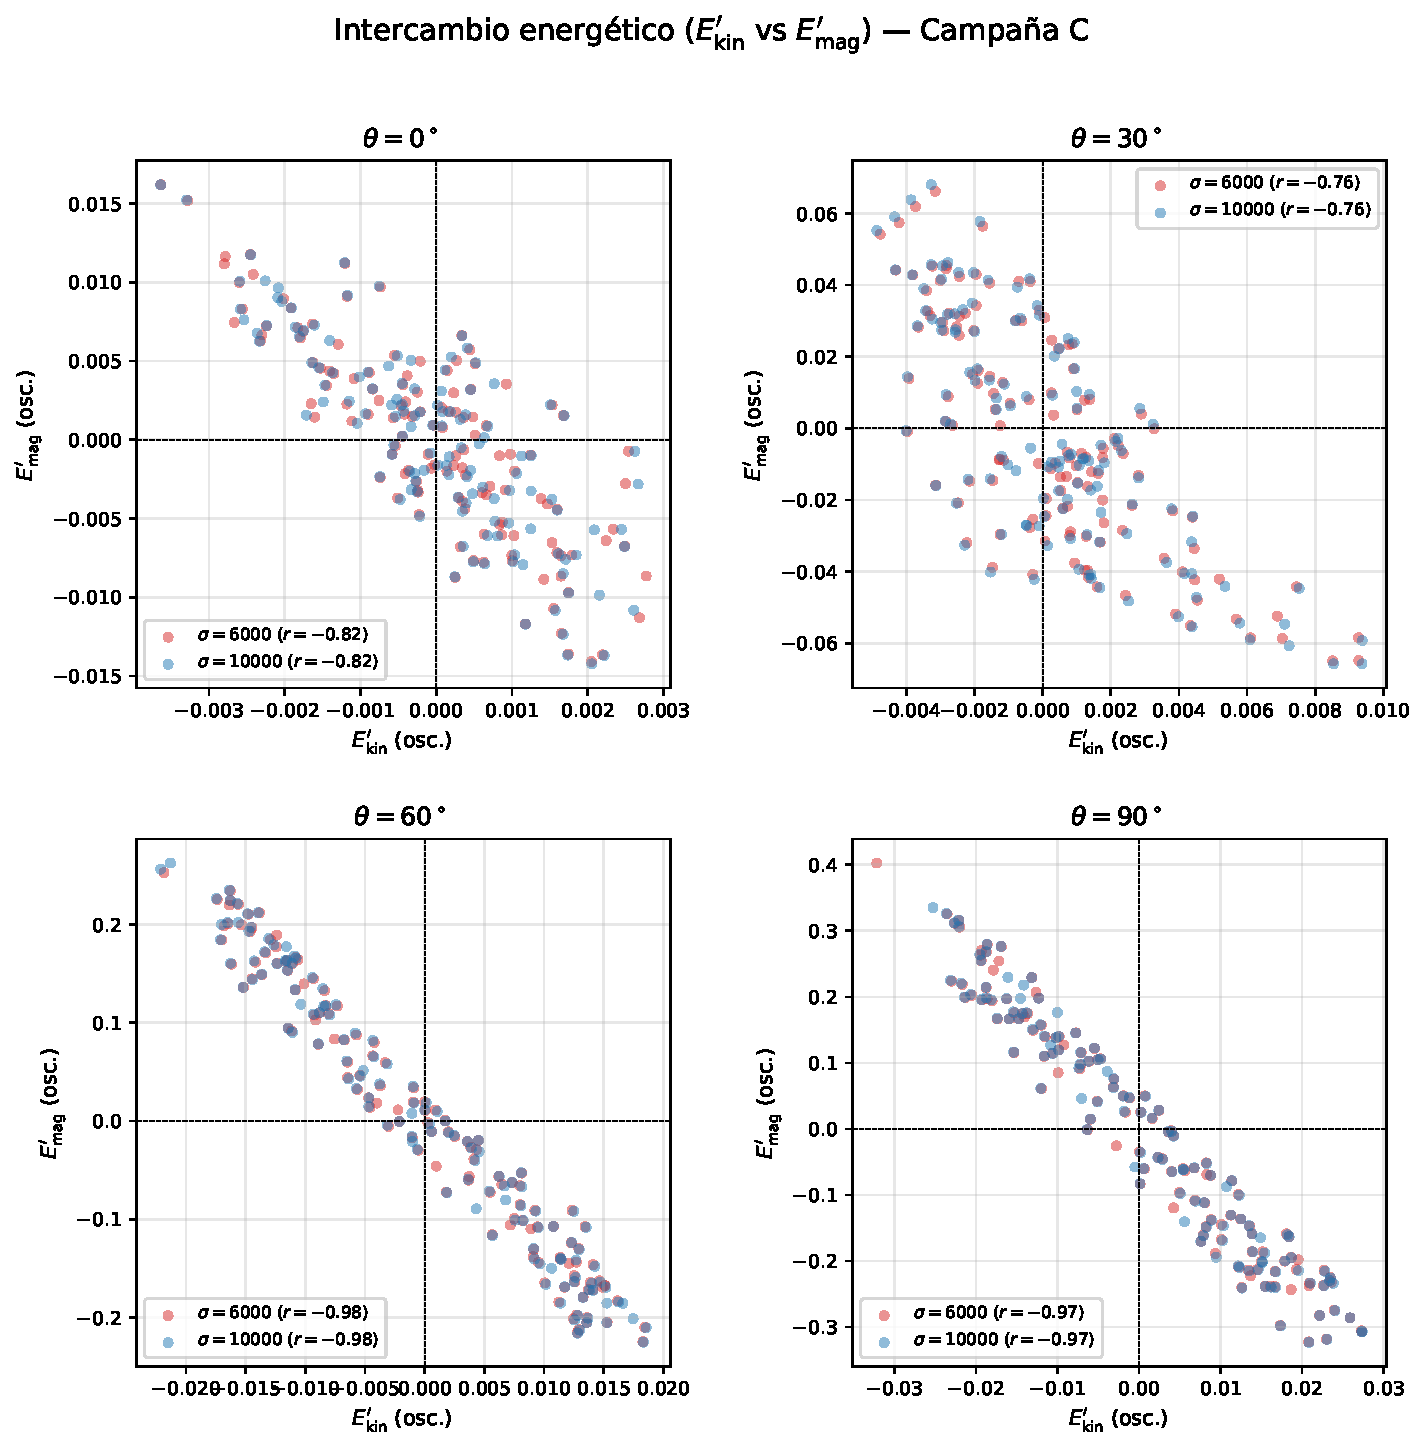
\includegraphics[width=0.96\linewidth,height=0.88\textheight,keepaspectratio]{fig_campC_ekin_emag_scatter.pdf}
\end{center}
\clearpage

\begin{center}
{\color{primary}\large\bfseries Figura 32}\quad{\small\color{accent}Respaldo B12}\quad{\small B12 · Mapas de Densidad de las Campa\~nas Magn\'eticas}\\[0.35cm]
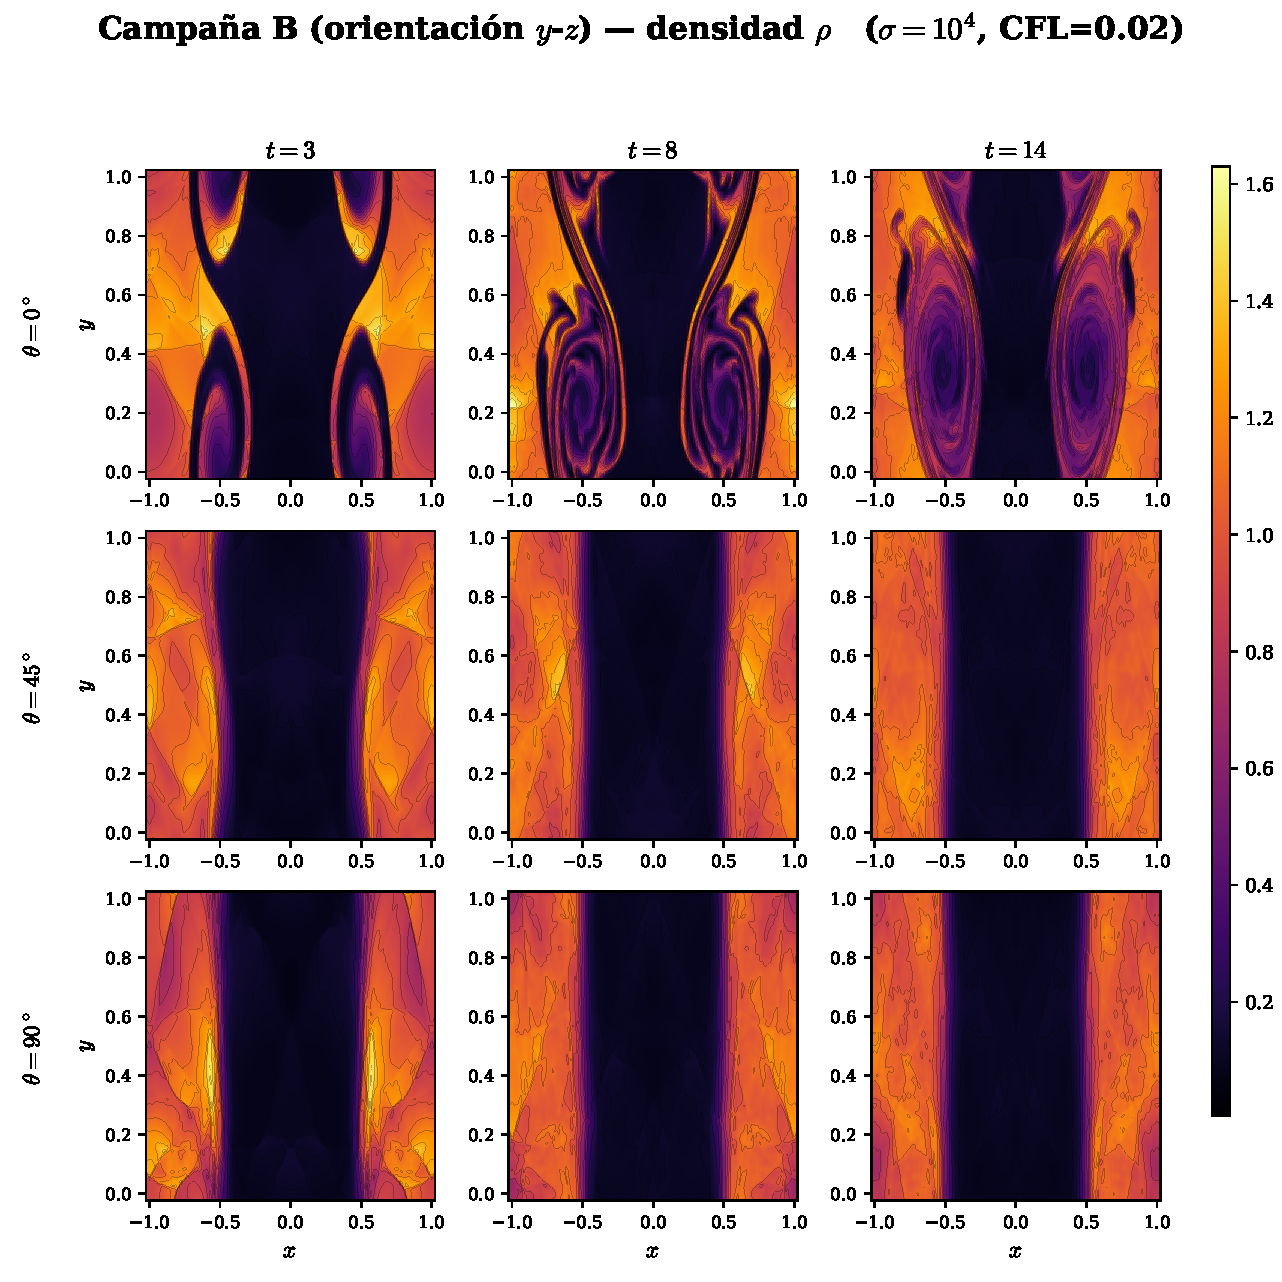
\includegraphics[width=0.96\linewidth,height=0.88\textheight,keepaspectratio]{fig_campB_rho_collage.pdf}
\end{center}
\clearpage

\begin{center}
{\color{primary}\large\bfseries Figura 33}\quad{\small\color{accent}Respaldo B12}\quad{\small B12 · Mapas de Densidad de las Campa\~nas Magn\'eticas}\\[0.35cm]
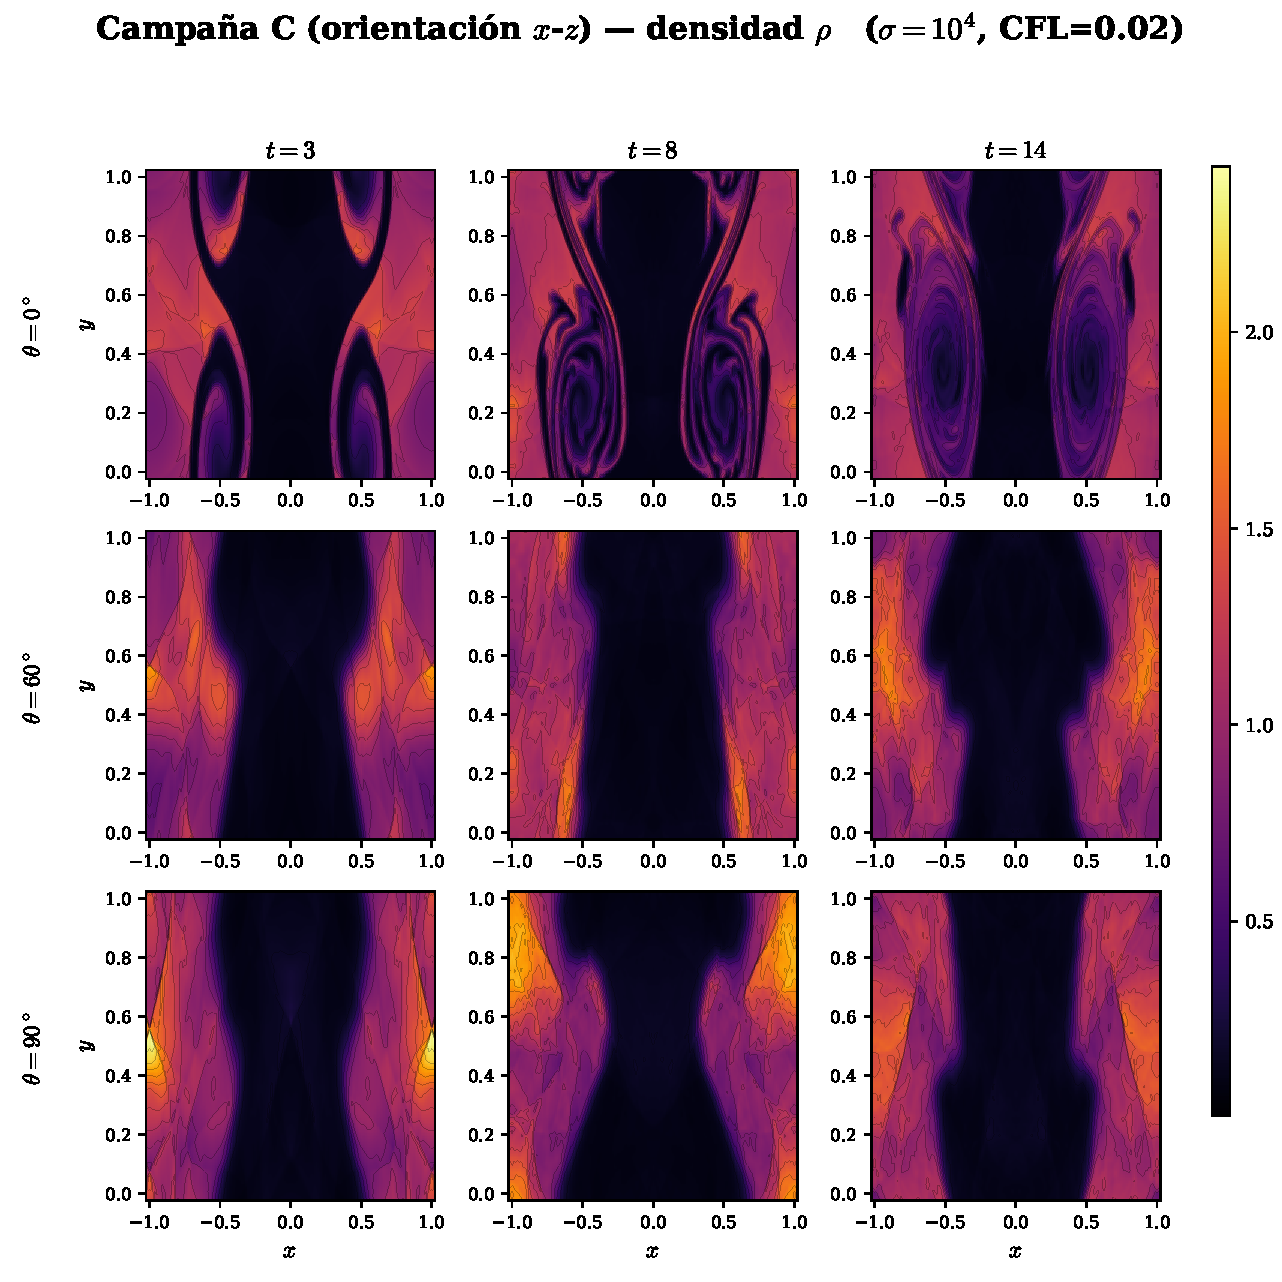
\includegraphics[width=0.96\linewidth,height=0.88\textheight,keepaspectratio]{fig_campC_rho_collage.pdf}
\end{center}
\clearpage

\begin{center}
{\color{primary}\large\bfseries Figura 34}\quad{\small\color{accent}Respaldo B13}\quad{\small B13 · Tablero Din\'amico de la Campa\~na B ($\sigma=6000$ vs $\sigma=10000$)}\\[0.35cm]
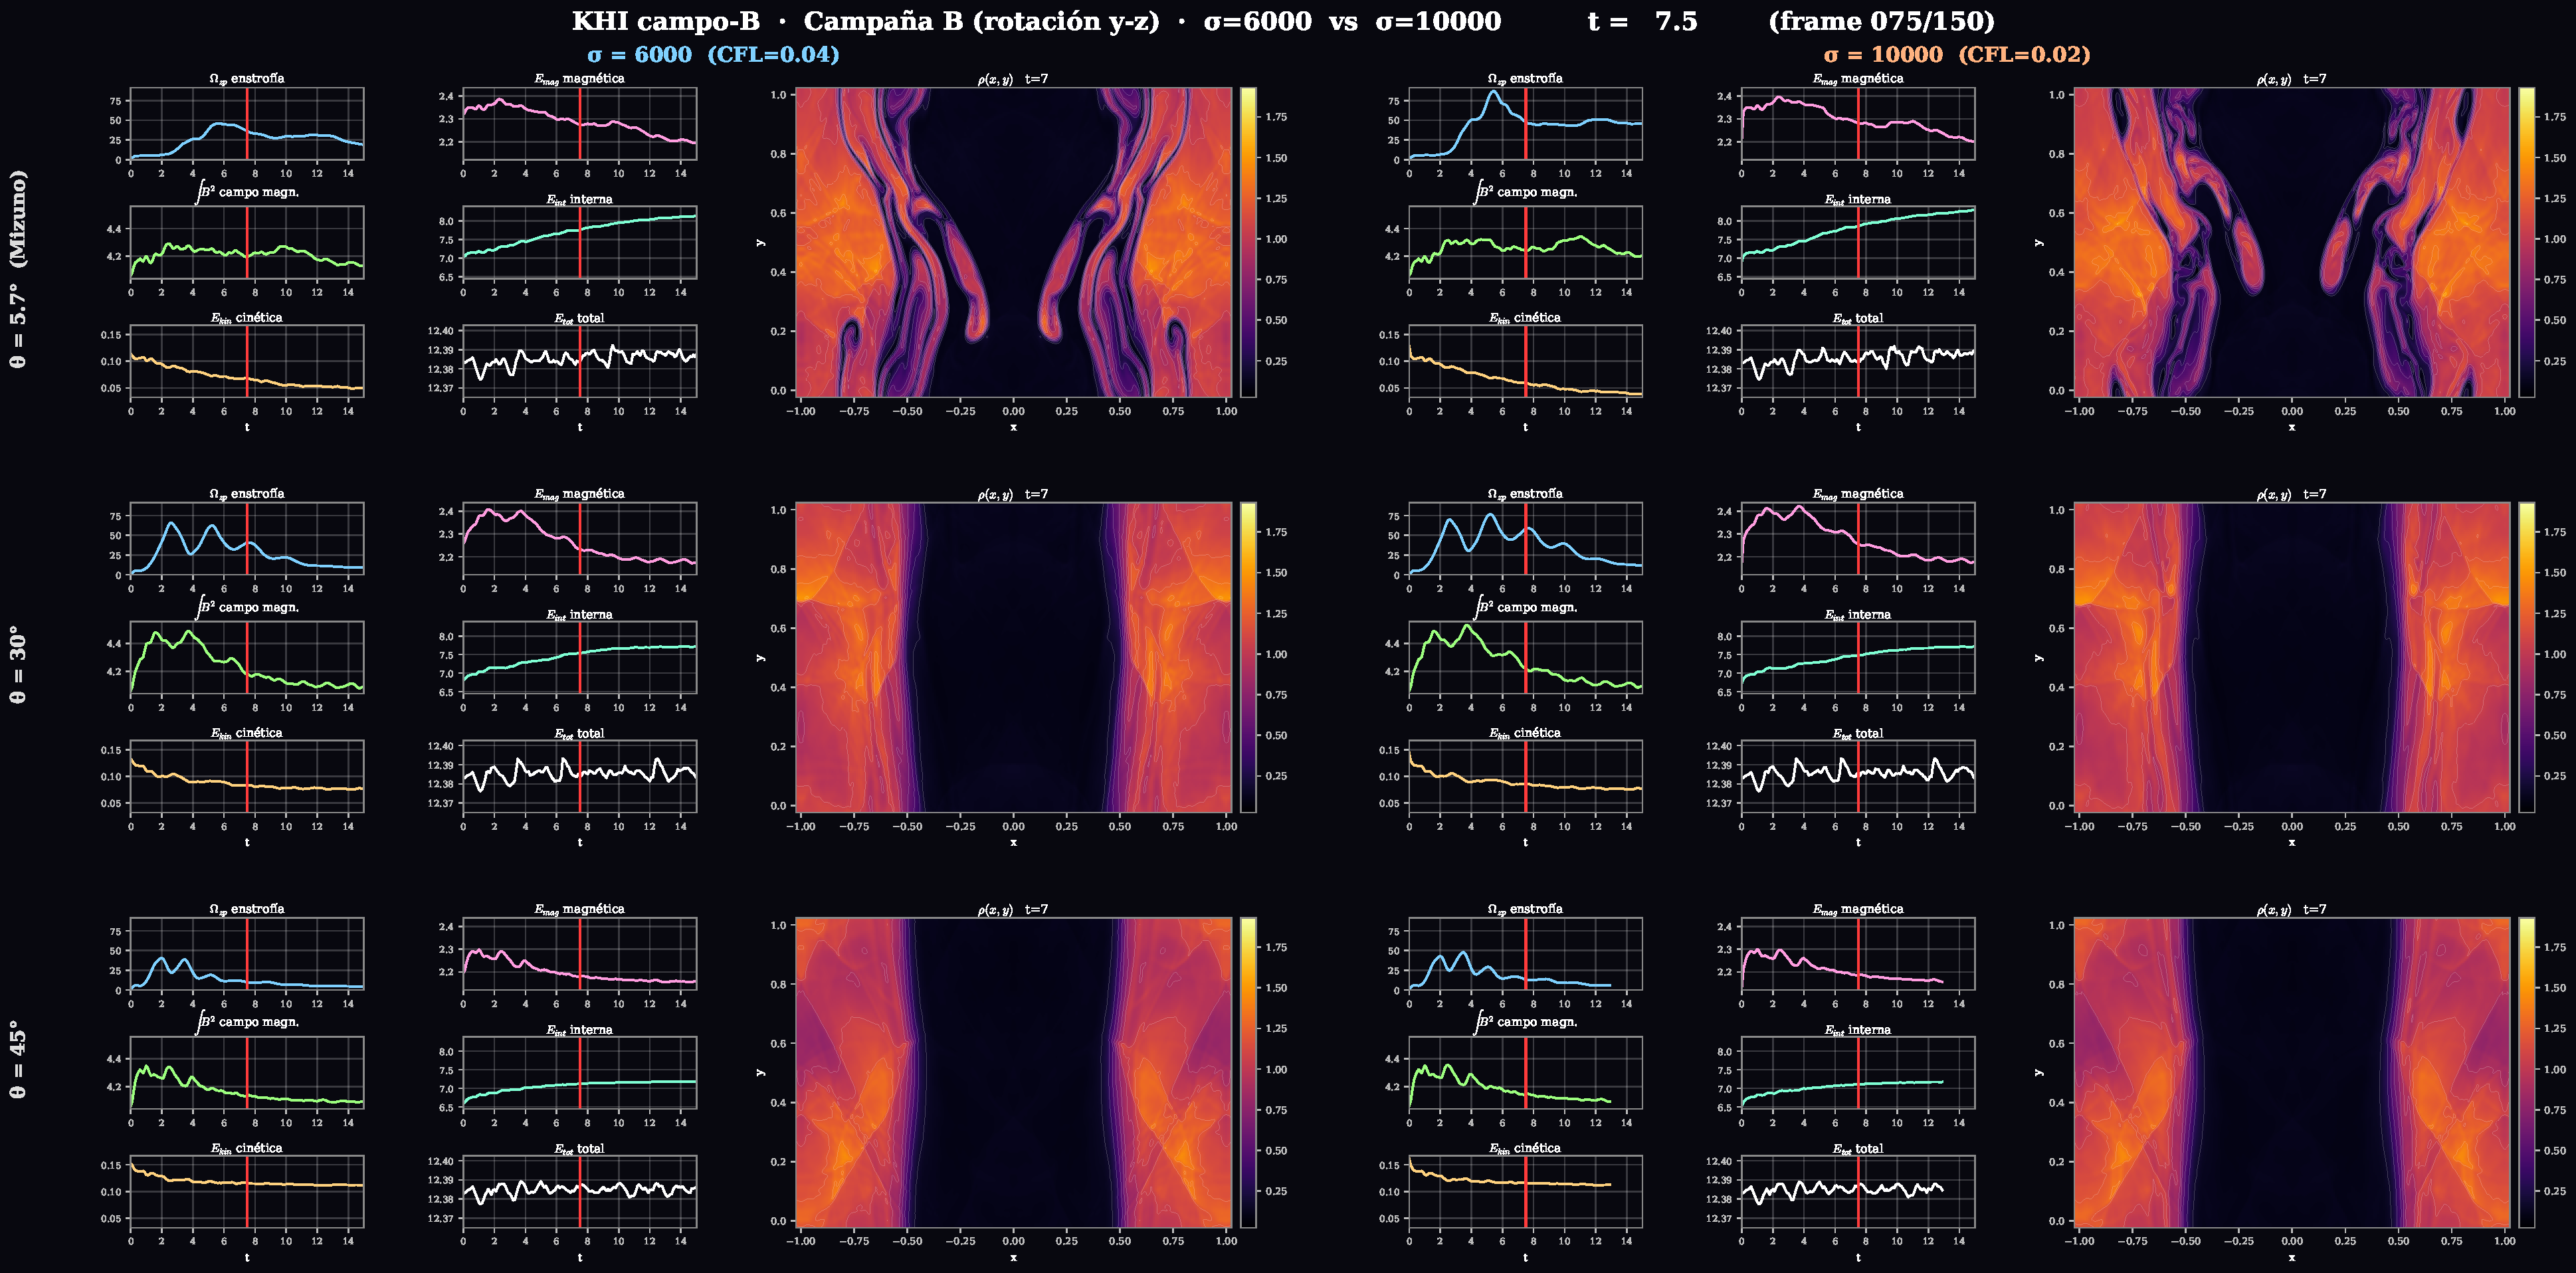
\includegraphics[width=0.96\linewidth,height=0.88\textheight,keepaspectratio]{campB_dashboard_t7p5.pdf}
\end{center}
\clearpage

\end{document}
